\documentclass[11pt]{book}

\tolerance=600

% for \begin{center}, etc.
\usepackage[margin=1.0in]{geometry}

\usepackage{seqsplit}

% all kinds of math macros
\usepackage{amsmath}
\usepackage{amssymb}

% eps figures
\usepackage{epsfig}

% chapter title styles
\usepackage[Sonny]{fncychap}
\ChNameVar{\LARGE}
\ChTitleVar{\LARGE\sl}

% index
\usepackage{makeidx}
\makeindex


% part page style see
% http://tex.stackexchange.com/questions/6609/problems-with-part-labels-using-titlesec
\usepackage{titlesec}

\titleformat{\part}[display]
   {\Huge\filcenter}
   {{\partname{}} \thepart}
   {0em}
   {\hrule}



% hyperlinks -- load after fncychap
\usepackage{hyperref}

% color package
\usepackage[usenames]{color}

% longtable package used to split tables across pages
\usepackage{longtable}

% PDF-aware landscape package, used for rotating tables (including the
% longtable)
\usepackage{pdflscape}

% table coloring
\usepackage{colortbl}
\definecolor{tableShade}{rgb}{0.945,0.961,0.980}


% make the MarginPars look pretty
\setlength{\marginparwidth}{0.75in}
\newcommand{\MarginPar}[1]{\marginpar{\vskip-\baselineskip\raggedright\tiny\sffamily
\hrule\smallskip{\color{red}#1}\par\smallskip\hrule}}

% to increase the likelihood that floats will occur "here" when you
% want them to
\renewcommand{\floatpagefraction}{1.0}
\renewcommand{\topfraction}{1.0}
\renewcommand{\bottomfraction}{1.0}
\renewcommand{\textfraction}{0.0}

% number subsubsections and put them in the TOC
\setcounter{tocdepth}{3}
\setcounter{secnumdepth}{3}

% custom hrule for title page
\newcommand{\HRule}{\rule{\linewidth}{0.125mm}}

% control sequences in verbatim
\usepackage{fancyvrb}

% short table of contents
\usepackage{shorttoc}

% spacing in the table of contents
\usepackage[titles]{tocloft}

\setlength{\cftbeforechapskip}{2ex}
\setlength{\cftbeforesecskip}{0.25ex}

% For splitting up lists into multitple columns
\usepackage{multicol}

% don't put a header on blank pages, see
% http://www.latex-community.org/forum/viewtopic.php?f=4&p=51559
% change ``plain'' to ``empty'' to eliminate the page number
\makeatletter
\renewcommand*\cleardoublepage{\clearpage\if@twoside
\ifodd\c@page\else
\hbox{}
\thispagestyle{empty}
\newpage
\if@twocolumn\hbox{}\newpage\fi\fi\fi}
\makeatother


% don't make the chapter/section headings uppercase.  See the fancyhdr
% documentation (section 9)
\usepackage{fancyhdr}
\renewcommand{\chaptermark}[1]{%
 \markboth{\chaptername
\ \thechapter.\ #1}{}}

\renewcommand{\sectionmark}[1]{\markright{\thesection---#1}}


% skip a bit of space between paragraphs, to enhance readability
\usepackage{parskip}



% special fraction
\newcommand{\sfrac}[2]{\mathchoice
  {\kern0em\raise.5ex\hbox{\the\scriptfont0 #1}\kern-.15em/
   \kern-.15em\lower.25ex\hbox{\the\scriptfont0 #2}}
  {\kern0em\raise.5ex\hbox{\the\scriptfont0 #1}\kern-.15em/
   \kern-.15em\lower.25ex\hbox{\the\scriptfont0 #2}}
  {\kern0em\raise.5ex\hbox{\the\scriptscriptfont0 #1}\kern-.2em/
   \kern-.15em\lower.25ex\hbox{\the\scriptscriptfont0 #2}}
  {#1\!/#2}}

\def\Ab {{\bf A}}
\def\eb {{\bf e}}
\def\Fb {{\bf F}}
\def\gb {{\bf g}}
\def\Hb {{\bf H}}
\def\ib {{\bf i}}
\def\Ib {{\bf I}}
\def\Kb {{\bf K}}
\def\lb {{\bf l}}
\def\Lb {{\bf L}}
\def\nb {{\bf n}}
\def\Pb {{\bf P}}
\def\Qb {{\bf Q}}
\def\rb {{\bf r}}
\def\Rb {{\bf R}}
\def\Sb {{\bf S}}
\def\ub {{\bf u}}
\def\Ub {{\bf U}}
\def\xb {{\bf x}}

\def\dt       {\Delta t}
\def\omegadot {\dot\omega}

\def\inp  {{\rm in}}
\def\outp {{\rm out}}
\def\sync {{\rm sync}}

\def\half   {\frac{1}{2}}
\def\myhalf {\sfrac{1}{2}}
\def\nph    {{n+\myhalf}}

% Level Set Macros
\def\ADDNODE       {{\tt{\bf ADDNODE}}}
\def\ADVANCE       {{\tt{\bf ADVANCE}}}
\def\done          {{\tt{\bf done}}}
\def\EVAL          {{\tt{\bf EVAL}}}
\def\INITPHI       {{\tt{\bf INITPHI}}}
\def\FASTMARCH     {{\tt{\bf FASTMARCH}}}
\def\FINDINTRFCE   {{\tt{\bf FINDINTRFCE}}}
\def\heap          {{\tt{\bf heap}}}
\def\heaploc       {{\tt{\bf heaploc}}}
\def\intface       {{\tt{\bf intface}}}
\def\intfacen      {{\tt{\bf intfacen}}}
\def\intfacenum    {{\tt{\bf intfacenum}}}
\def\intfacenumn   {{\tt{\bf intfacenumn}}}
\def\intfacenump   {{\tt{\bf intfacenump}}}
\def\intfacep      {{\tt{\bf intfacep}}}
\def\isnew         {{\tt{\bf isnew}}}
\def\LARGEINT      {{\tt{\bf LARGEINT}}}
\def\lvlerr        {{\tt{\bf lvlerr}}}
\def\LSCFL         {{\tt{\bf LSCFL}}}
\def\LStype        {{\tt{\bf LStype}}}
\def\LSnband       {{\tt{\bf LSnband}}}
\def\LSmine        {{\tt{\bf LSmine}}}
\def\mine          {{\tt{\bf mine}}}
\def\MINE          {{\tt{\bf MINE}}}
\def\mineloc       {{\tt{\bf mineloc}}}
\def\NARROWBAND    {{\tt{\bf NARROWBAND}}}
\def\nband         {{\tt{\bf nband}}}
\def\nbandnum      {{\tt{\bf nbandnum}}}
\def\nbandwidth    {{\tt{\bf nbandwidth}}}
\def\numtent       {{\tt{\bf numtent}}}
\def\PHIUPD        {{\tt{\bf PHIUPD}}}
\def\REINIT        {{\tt{\bf REINIT}}}
\def\RETYPIFY      {{\tt{\bf RETYPIFY}}}
\def\RMVNODE       {{\tt{\bf RMVNODE}}}
\def\sign          {{\tt{\bf sign}}}
\def\type          {{\tt{\bf type}}}
\def\UPDATE        {{\tt{\bf UPDATE}}}
\def\UPDATEF       {{\tt{\bf UPDATEF}}}
\def\UPDATENODE    {{\tt{\bf UPDATENODE}}}
\def\new           {{\rm new}}
\def\old           {{\rm old}}


\usepackage{listings}

\definecolor{gray}{rgb}       {0.8,0.8,0.8}
\definecolor{light-blue}{rgb} {0.8,0.8,1.0}
\definecolor{light-green}{rgb}{0.8,1.0,0.8}
\definecolor{light-red}{rgb}  {1.0,0.9,0.9}

\lstset{frame=single,basicstyle=\footnotesize\ttfamily,showstringspaces=false,showspaces=false,xleftmargin=5pt,xrightmargin=6pt}

\lstset{language=C++,
                basicstyle=\footnotesize\ttfamily,
                keywordstyle=\color{blue}\footnotesize\ttfamily,
                commentstyle=\color{cyan}\footnotesize\ttfamily
}

\lstdefinelanguage{cpp}{
  language     = C++,
  morekeywords = [2]{amrex,IntVect,Array,IndexType,Box,BaseFab,FArrayBox,IArrayBox,BoxArray,DistributionMapping,ParallelDescriptor,FabArray,MultiFab,MFIter,BL_SPACEDIM,D_DECL},
  keywordstyle = [2]\color{red}\footnotesize\ttfamily,
}

% \lstset{
%   basicstyle=\small\ttfamily,%
%   frame=single,%
%   rulesepcolor=\color{gray},%
%   backgroundcolor=\color{white}%
% }
% \lstset{belowskip=-0.25em}


% Macros for indexing
\newcommand{\idxamrex}[1]{\index{\tt{amrex}!{\tt #1}}{\tt #1}}

%------------------------------------------------------------------------------
\input amrexsymbols
% \graphicspath{{Verification/}{Software/}{ConvertCheckpoint/}{Scaling/}{Visualization/}}


%------------------------------------------------------------------------------
\begin{document}



\frontmatter

\begin{titlepage}
\begin{center}
\ \\[3in]
{\sf \Huge AMReX}
\ \\[0.2in]

\begin{minipage}{5.5in}
\HRule\\[2mm]
\centering
{\Large \em An adaptive mesh refinement software framework}

\HRule
\end{minipage}

\ \\[.5 in]
{\sf \huge User's Guide}

\vfill

{\large AMReX Developers}
\ \\[0.3 in]
{\large \today}
\end{center}

\end{titlepage}


\shorttoc{Chapter Listing}{0}

\setcounter{tocdepth}{2}
\tableofcontents

\clearpage

\listoffigures
\addcontentsline{toc}{chapter}{list of figures}

\clearpage

\listoftables
\addcontentsline{toc}{chapter}{list of tables}


\cleardoublepage

\chapter*{Preface}
\addcontentsline{toc}{chapter}{Preface}
\noindent The current version of the \BoxLib\ User's Guide can be found in 
the \BoxLib\ git repository in {\tt BoxLib/docs}.  Visit our website
at {\tt https://ccse.lbl.gov} for free access to \BoxLib.  Any questions,
comments, suggestions, etc., regarding this User's Guide should be directed
to Andy Nonaka of CCSE at {\tt AJNonaka@lbl.gov}.  Further information 
about \BoxLib\ can be found by contacting Ann Almgren of CCSE at 
{\tt ASAlmgren@lbl.gov} or by visiting our website.\\

\noindent (c) 1996-2000 The Regents of the University of California (through
E.O. Lawrence Berkeley National Laboratory), subject to approval by
the U.S. Department of Energy.  Your use of this software is under
license -- the license agreement is attached and included in the
\BoxLib\ home directory as license.txt or you may contact Berkeley Lab's Technology
Transfer Department at TTD@lbl.gov.  NOTICE OF U.S. GOVERNMENT RIGHTS.
The Software was developed under funding from the U.S. Government
which consequently retains certain rights as follows: the
U.S. Government has been granted for itself and others acting on its
behalf a paid-up, nonexclusive, irrevocable, worldwide license in the
Software to reproduce, prepare derivative works, and perform publicly
and display publicly.  Beginning five (5) years after the date
permission to assert copyright is obtained from the U.S. Department of
Energy, and subject to any subsequent five (5) year renewals, the
U.S. Government is granted for itself and others acting on its behalf
a paid-up, nonexclusive, irrevocable, worldwide license in the
Software to reproduce, prepare derivative works, distribute copies to
the public, perform publicly and display publicly, and to permit
others to do so.\\



\mainmatter

\chapter{Introduction}\label{Chap:Introduction}
\section{What is \BoxLib?}

\BoxLib\ is a software library containing all the functionality to write massively parallel, 
block-structured adaptive mesh refinement (AMR) applications in two and three dimensions.
\BoxLib\ was developed at the Center for Computational Sciences and Engineering (CCSE) at 
Lawrence Berkeley National Laboratory and is freely available
at {\tt https://github.com/BoxLib-Codes/BoxLib}.  The most current version of this User's Guide
can be found in the \BoxLib\ git repository at {\tt BoxLib/Docs}.  Any questions,
comments, suggestions, etc., regarding this User's Guide should be directed
to Andy Nonaka of CCSE at {\tt AJNonaka@lbl.gov}.  Further information 
about \BoxLib\ can be found by contacting Ann Almgren of CCSE at 
{\tt ASAlmgren@lbl.gov} or by visiting our website.\\

If you are new to \BoxLib, we recommend you read Chapters \ref{Chap:Introduction} and
\ref{Chap:Getting Started} and familiarize yourself with the accompanying tutorial code.
After working through Chapter \ref{Chap:Getting Started}, you will be able to run the tutorial
code on as many cores as you like!  Then, in Chapter \ref{Chap:Advanced Topics F} we enhance 
the Fortran90 tutorial code with additional features.

\section{High-Level Overview}

Key features of \BoxLib\ include:
\begin{itemize}
\item C++/Fortran90 and pure Fortran90 versions
\item Optional subcycling in time 
\item Support for cell-centered, face-centered, edge-centered, and nodal data
\item Support for hyperbolic, parabolic, and elliptic solves on hierarchical grid structure
\item Supports hybrid MPI/OpenMP parallel programming model
\item Demonstrated scaling of linear solvers (parabolic and elliptic solvers) to 100,000 processors and 
      hydrodynamics (hyperbolic solvers) to over 200,000 processors
\item Plotfile format can be read by {\tt VisIt}, {\tt yt}, and {\tt AmrVis}
\item Basis of mature applications in combustion, astrophysics, cosmology, porous media, and fluctuating hydrodynamics
\item Freely available at {\tt https://github.com/BoxLib-Codes/BoxLib}
\end{itemize}

\subsection{Parallel Programming Model}

The fundamental parallel abstraction in \BoxLib\ is the \MultiFab, which holds the data on the 
union of grids at a level of refinement.  A \MultiFab\ is composed of multiple ``Fortran array boxes''
(i.e., \FArrayBox es or \Fab s); each \Fab\ is a multidimensional array of data on a single grid. 
Whenever ``work'' needs to be done using data from a \MultiFab, the 
\Fab s composing that \MultiFab\ are distributed among different processors 
to be worked on simultaneously.  \Fab s at each level of refinement are distributed 
independently.  The software supports two data distribution schemes, as well as a 
dynamic switching scheme that decides which approach to use based on the number of 
grids at a level and the number of processors.  The first scheme is based on a 
heuristic knapsack algorithm, which emphasizes load balancing; the second is based on 
the use of a Morton-ordering space-filling curve, which emphasizes on data locality for
faster grid-to-grid communication. 
\MultiFab\ operations are performed with an ``owner computes'' rule 
with each processor operating independently on its local data.  For operations that 
require data owned by other processors, the \MultiFab\ operations are preceded by a 
data exchange between processors to fill ghost cells.  Each processor contains 
meta-data that is needed 
to fully specify the data locality and processor assignments of the \Fab s. At a 
minimum, this requires the storage of an array of coordinates specifying the index space 
region for each box at each level of refinement.  The meta-data can thus be used to 
dynamically evaluate the necessary communication patterns for sharing data amongst 
processors, enabling us to optimize communications patterns within the algorithm.
By using a hybrid MPI-OpenMP approach to parallelization (see below), we are able to 
compute with fewer, larger grids, and thus the size of the meta-data is substantially 
reduced.

\subsection{Hybrid MPI--OpenMP}

The basic parallelization strategy uses a hierarchical programming approach for 
multicore architectures based on both MPI and OpenMP.  In the pure-MPI instantiation, 
each \Fab\ is assigned to a core, and each core communicates 
with every other core using only MPI.  In the hybrid approach, where on each socket/node 
there are $n$ cores that all access the same memory, we can divide our domain into
fewer, larger grids, and assign each \Fab\ to a socket/node, 
with the work associated with that grid distributed among the $n$ 
cores using OpenMP.

\subsection{Parallel I/O}

Data for checkpoints and analysis are written in a self-describing format that consists 
of a directory for each time step written. Checkpoint directories contain all necessary 
data to restart the calculation from that time step. Plotfile directories contain data 
for post-processing, visualization, and analytics, which can be read using {\tt VisIt}, 
{\tt yt}, or {\tt AmrVis} (a customized visualization package developed at CCSE for 
visualizing data on AMR grids, also freely available on our website).  Within each 
checkpoint or plotfile directory is an ASCII header file and a
subdirectory for each AMR level.  The header describes the AMR hierarchy, including 
number of levels, the grids at each level, the problem size, refinement ratio 
between levels, time step, time, etc.  Each of the subdirectories contains the data 
associated with the \MultiFab\ for that level, which is stored in multiple files.
Checkpoint and plotfile directories are written at user-specified intervals.\\

Restarting a calculation can present some difficult issues for reading data efficiently. 
In the worst case, all processors would need data from all files. If multiple processors 
try to read from the same file at the same time, performance problems can result, with 
extreme cases causing file system thrashing.  Since the number of files is generally not 
equal to the number of processors and each processor may need data from multiple files, 
input during restart is coordinated to efficiently read the data. Each data file is only 
opened by one processor at a time. The {\tt IOProcessor} creates a database for mapping files 
to processors, coordinates the read queues, and interleaves reading its own data.  Each 
processor reads all data it needs from the file it currently has open.  The code tries to 
maintain the number of input streams to be equal to the number of files at all times. 
Checkpoint and plotfiles are portable to machines with a different byte ordering and 
precision from the machine that wrote the files.  Byte order and precision translations 
are done automatically, if required, when the data is read.

\subsection{Scaling}

In Figure \ref{fig:scaling} we present weak scaling results for several of our codes on 
the Cray XT5 Jaguarpf at OLCF. Jaguarpf has two hex-core sockets on each node. We assign 
one MPI process per node and spawn a single thread on each of the 12 cores. Results are 
shown for our compressible astrophysics code, {\tt CASTRO}; the low Mach number code, 
{\tt MAESTRO}; and our low Mach number combustion code, {\tt LMC}. In the {\tt MAESTRO} 
and {\tt CASTRO} tests, we simulate a full spherical star on a 3D grid with one refined 
level (2 total levels).  {\tt LMC} is tested on a 3D methane flame with detailed chemistry 
using two refined levels. {\tt MAESTRO} and {\tt LMC} scale well to 50K-100K cores, 
whereas {\tt CASTRO} scales well to over 200K cores. The overall scaling behavior 
for {\tt MAESTRO} and {\tt LMC} is not as close to ideal as that of {\tt CASTRO} 
due to the communication-intensive linear solves performed at each time step. However, 
these low Mach number codes are able to take a much larger time step than explicit 
compressible formulations in the low Mach number regime. 
%%%%%%%%%%%%%%%%%%%%%%%%%%%%%%%%%%%%%
\begin{figure}[tb]
\centering
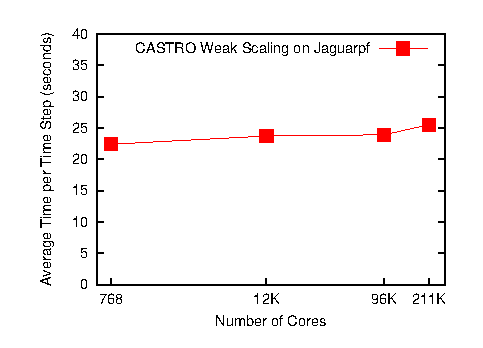
\includegraphics[width=3in]{./Introduction/castro_scaling}
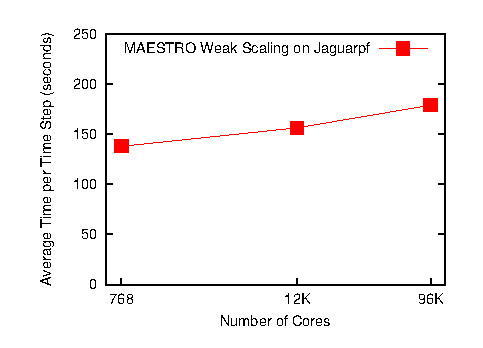
\includegraphics[width=3in]{./Introduction/maestro_scaling}
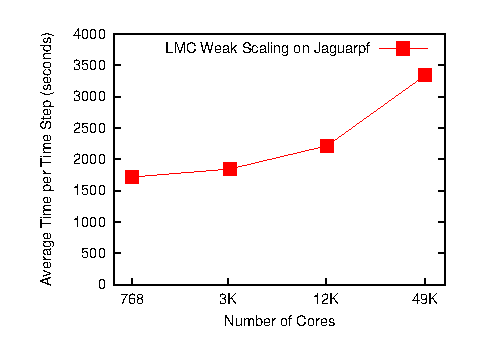
\includegraphics[width=3in]{./Introduction/lmc_scaling}
\caption{\label{fig:scaling}Weak scaling results for {\tt CASTRO}, {\tt MAESTRO}, and
{\tt LMC} on the Cray XT5 Jaguarpf at OLCF.}
\end{figure}
%%%%%%%%%%%%%%%%%%%%%%%%%%%%%%%%%%%%%

\section{\BoxLib\ Directory Structure}

\BoxLib\ is the base directory in a hierarchy of subdirectories that
support parallel, block-structured AMR applications in C++ and Fortran90.
A schematic of the \BoxLib\ directory structure is shown in Figure 
\ref{fig:boxlib_directory}.
%%%%%%%%%%%%%%%%%%%%%%%%%%%%%%%%%%%%%
\begin{figure}[tb]
\centering
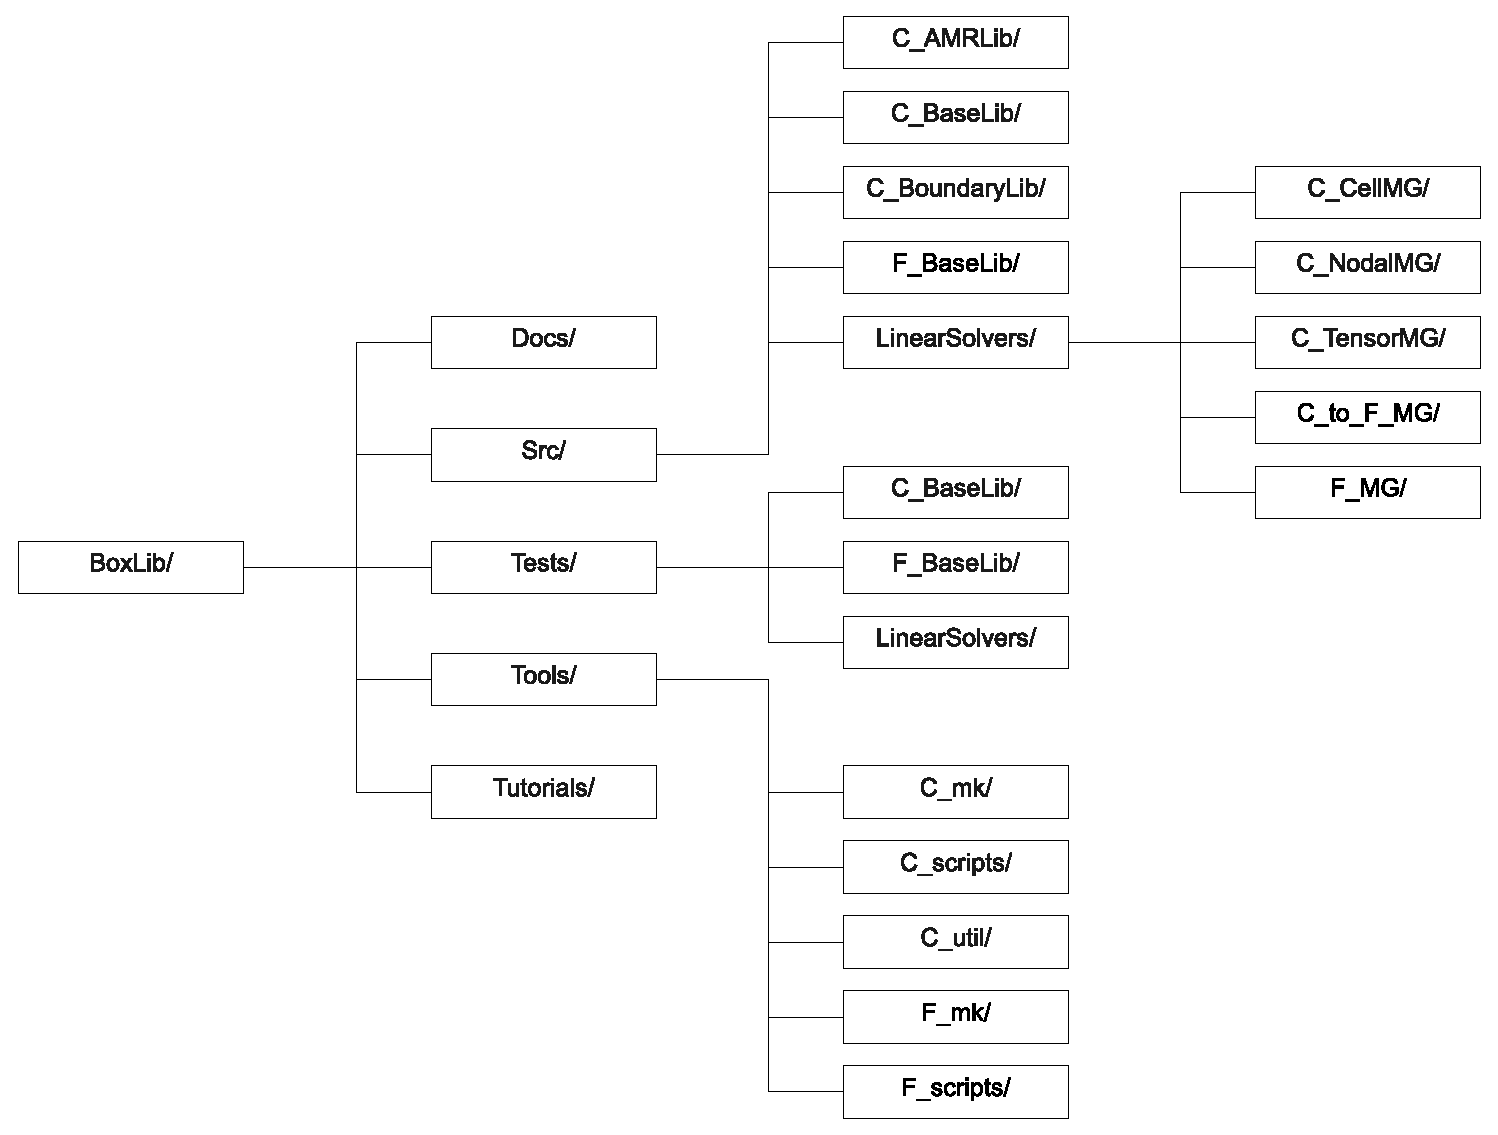
\includegraphics[width=6.5in]{./Introduction/boxlib_directory_bw2}
\caption{\label{fig:boxlib_directory}\BoxLib\ directory structure.}
\end{figure}
%%%%%%%%%%%%%%%%%%%%%%%%%%%%%%%%%%%%%

\begin{itemize}

\item {\tt Docs/}

Contains this \BoxLib\ User's Guide.

\item {\tt Src/}

  \BoxLib\ source code.  The C++ source code is split into several directories.
  The Fortran90 source code is contained in one directory.

  \begin{itemize}

    \item {\tt C\_AMRLib/}
    \item {\tt C\_BaseLib/}
    \item {\tt C\_BoundaryLib/}
    \item {\tt F\_BaseLib/}
    \item {\tt LinearSolvers/}

    Source code for various linear solvers in C++ and Fortran90.

    \begin{itemize}

      \item {\tt C\_CellMG/}
      \item {\tt C\_NodalMG/}
      \item {\tt C\_TensorMG/}
      \item {\tt C\_to\_F\_MG/}
      \item {\tt F\_MG/}

    \end{itemize}

  \end{itemize}

\item {\tt Tests/}

  Various tests used by \BoxLib\ developers.

  \begin{itemize}

  \item {\tt C\_BaseLib/}
  \item {\tt F\_BaseLib/}
  \item {\tt LinearSolvers/}

  \end{itemize}

\item {\tt Tools/}

  \begin{itemize}

  \item {\tt C\_mk/}

  The generic Makefiles that store the C++ compilation flags for
  various platforms.

  \item {\tt C\_scripts/}

  Some simple scripts that are useful for building, running,
  maintaining codes in C++.

  \item {\tt C\_Util/}

  Various utility codes for analyzing plotfiles.

  \item {\tt F\_mk/}

  The generic Makefiles that store the Fortran90 compilation flags for
  various platforms.

  \item {\tt F\_scripts/}

  Some simple scripts that are useful for building, running,
  maintaining codes in Fortran90.

  \end{itemize}

\item {\tt Tutorials/}

  Contains sample codes referred to in this User's Guide.

\end{itemize}


\chapter{Getting Started}\label{Chap:GettingStarted}
We now give an overview of common data structures used in \BoxLib, followed by a simple
example written in both Fortran90 and C++ that makes use of these structures.
The example advances two scalar variables in time on a single level with multiple 
grids (no AMR) and produces plotfiles.

\section{Overview of Data Structures}

\BoxLib\ contains the most fundamental objects used to construct parallel
block-structured AMR applications.
At each level of refinement, the region covered by that level is divided
into grids, or boxes.  The entire computational domain is covered by
the coarsest (base) level of refinement (called level $\ell=0$ in C++ 
and called level $\ell=1$ in Fortran90) and can be represented on one
grid or divided into many grids.
Higher levels of refinement have cells that are finer by a ``refinement ratio''
of either 2 or 4 (in C++) or 2 (in Fortran90).  The grids are properly nested in the sense that the union 
of grids at level $\ell+1$ is contained in the union of grids at level $\ell$.
Furthermore, the containment is strict in the sense that, except at physical 
boundaries (i.e., domain boundaries that are not periodic),
the level $\ell$ grids are large enough to guarantee that there is
a border at least $n_{\rm buffer}$ (typically 4) level $\ell$ cells wide surrounding each level
$\ell +1$ grid (grids at all levels are allowed to extend to the physical
boundaries so the proper nesting is not strict there).  See Figure \ref{fig:AMR}
for a sample two-dimensional grid structure.\\
%%%%%%%%%%%%%%%%%%%%%%%%%%%%%%%%%%%%%
\begin{figure}[tb]
\centering
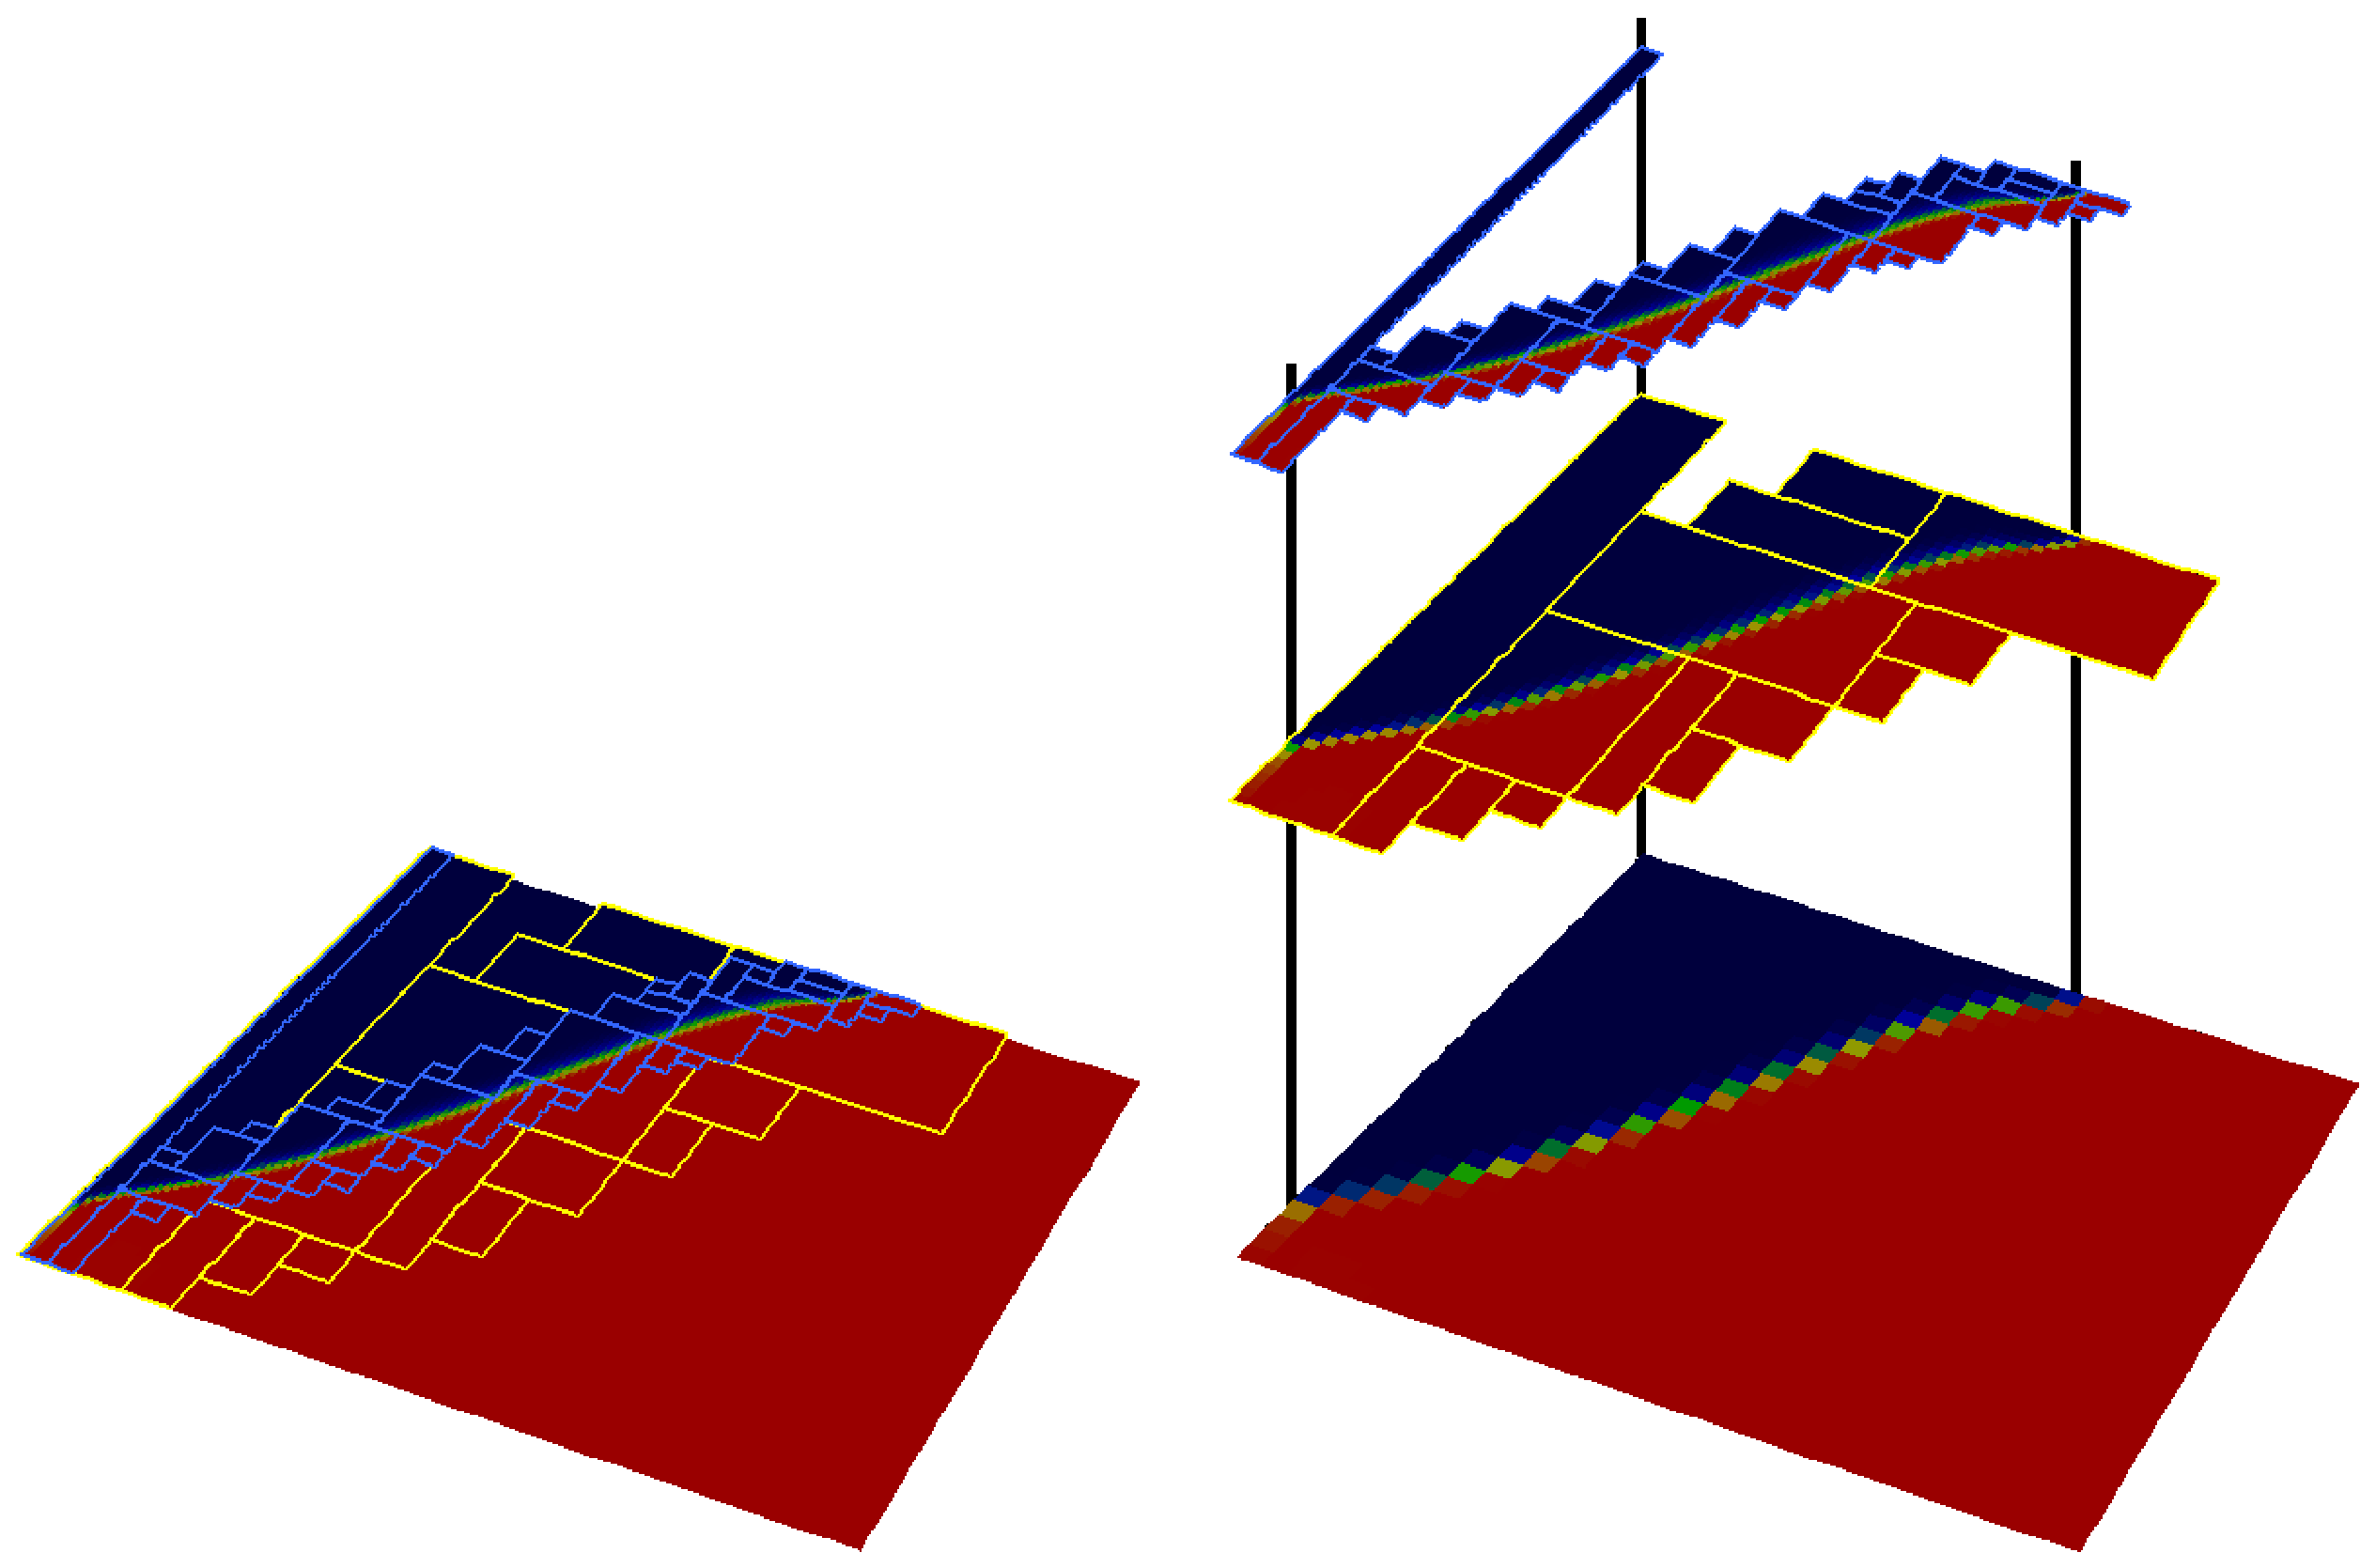
\includegraphics[width=6.5in]{./Introduction/AMR}
\caption{\label{fig:AMR}Sample grid structure with two levels of refinement.  These
grids satisfy the requirements that the base grid covers the entire computational domain 
and the grids are properly nested.  Note that refined grids are allowed to extend to physical
domain boundaries without coarser buffer cells.}
\end{figure}
%%%%%%%%%%%%%%%%%%%%%%%%%%%%%%%%%%%%%

On a grid, the data can be stored at cell-centers, faces, edges, or
corners.  In \BoxLib, data that is on an face is termed `nodal'
in that one direction (see Figure~\ref{fig:dataloc}).  In three-dimensions (not pictured),
data that is nodal in two directions is said to live on edges.  Data that is nodal in
all directions lives on the corners of cells (commonly referred to as the nodes).
\BoxLib\ uses $0$-based spatial indexing, and for data that is nodal in one or more direction,
the integer index corresponds to the lower boundary in that direction (see Figure~\ref{fig:dataloc}).
In our \BoxLib\ applications, the state data (velocity, density, 
species, $\ldots$) is typically cell-centered.  Fluxes are typically nodal in exactly
one direction (i.e.~they are face-centered).  A few quantities are nodal in all 
directions (e.g.~the pressure in the low Mach number projection methods).
%%%%%%%%%%%%%%%%%%%%%%%%%%%%%%%%%%%%%
\begin{figure}[tb]
\centering
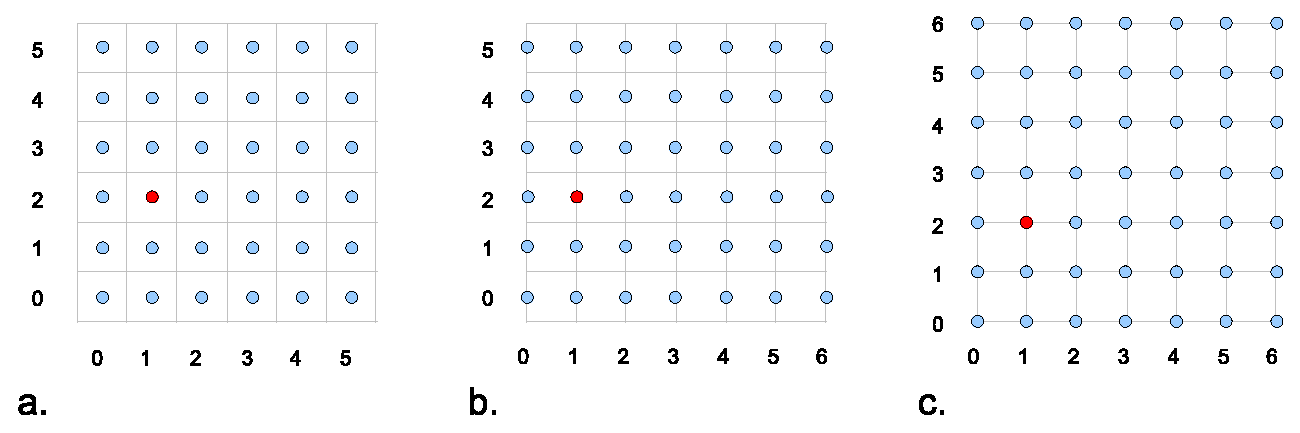
\includegraphics[width=6.5in]{./Introduction/data_loc2}
\caption{\label{fig:dataloc} Some of the different data-centerings in two dimensions:
(a) cell-centered, (b) nodal in the $x$-direction only (face-centered), and (c) nodal in
both the $x$- and $y$-directions.  Note that for data that is nodal in one or more direction,
the integer index corresponds to the lower boundary in that direction.
Also note that \BoxLib\ uses $0$-based indexing, e.g., in each of these centerings, 
the red point has the same indices:\ (1,2).
Not shown is the case where data is nodal in the $y$-direction only.  
Also not shown is the three-dimensional edge-centered case, where the data
is nodal in exactly two directions.  }
\end{figure}
%%%%%%%%%%%%%%%%%%%%%%%%%%%%%%%%%%%%%

\begin{itemize}
\item In C++ \BoxLib, we must specify the number of spatial dimensions (1, 2, or 3), 
{\tt DIM}, at compile-time.  The code that will be built is specifically designed to 
run only with that number of dimensions.
\item In Fortran90 \BoxLib, we build dimension-independent code at compile-time, 
and tell the program the dimensionality of the problem via a runtime inputs file.
\end{itemize}

To simplify the description of the underlying AMR grid, \BoxLib\
provides a number of classes.  We now briefly summarize some of the major
classes.

\subsection{\IntVect}

\IntVect s are {\tt DIM}-tuples of integers that are used to define
indices in space.  In C++, an example of an \IntVect\ in 2D would be
(C++ source code will be shaded blue):
\begin{lstlisting}[backgroundcolor=\color{light-blue}]
IntVect iv(3,5);
\end{lstlisting}
In Fortran90, we don't use \IntVect s, but instead use standard
arrays of integers (Fortran90 source code will be shaded green):
\begin{lstlisting}[backgroundcolor=\color{light-green}]
integer :: iv(2)
iv(1) = 3
iv(2) = 5
\end{lstlisting}

\subsection{\BoxType}

A \BoxType\ is simply a rectangular domain in space and does not hold any data.
A \BoxType\ contains the indices of its low end and high end, 
{\tt IntVect lo} and {\tt IntVect hi}.
\begin{itemize}
\item In C++, a \BoxType\ also
contains an {\tt IndexType} (cell-centered, face-centered, or nodal) for each
spatial direction.
\item In Fortran90, a \BoxType\ also contains the dimensionality 
of the \BoxType.
\end{itemize}
To build a \BoxType\ in C++ use:
\begin{lstlisting}[backgroundcolor=\color{light-blue}]
IntVect iv_lo(0,0);
IntVect iv_hi(15,15);
Box bx(iv_lo,iv_hi);
\end{lstlisting}
To build a \BoxType\ in Fortran90 use:
\begin{lstlisting}[backgroundcolor=\color{light-green}]
type(box) :: bx
integer   :: iv_lo(2), iv_hi(2)
iv_lo(1:2) = 0
iv_hi(1:2) = 15
bx = make_box(lo,hi)
\end{lstlisting}

The computational domain is divided into non-overlapping grids.  
The collection of grids at the same resolution comprise a level.
Figure~\ref{fig:boxes} shows three grids at the same level of
refinement.  Note that this figure cannot represent the base level of refinement,
since it would require that the grids span the problem domain.
The position of the grids is with respect to a global
index space that covers the entire domain at that level and uses 0-based indexing.
For example, the \BoxType\ associated with grid 1 
in the figure has {\tt lo} = (2,6) and {\tt hi} = (5,13).
%%%%%%%%%%%%%%%%%%%%%%%%%%%%%%%%%%%%%
\begin{figure}[tb]
\centering
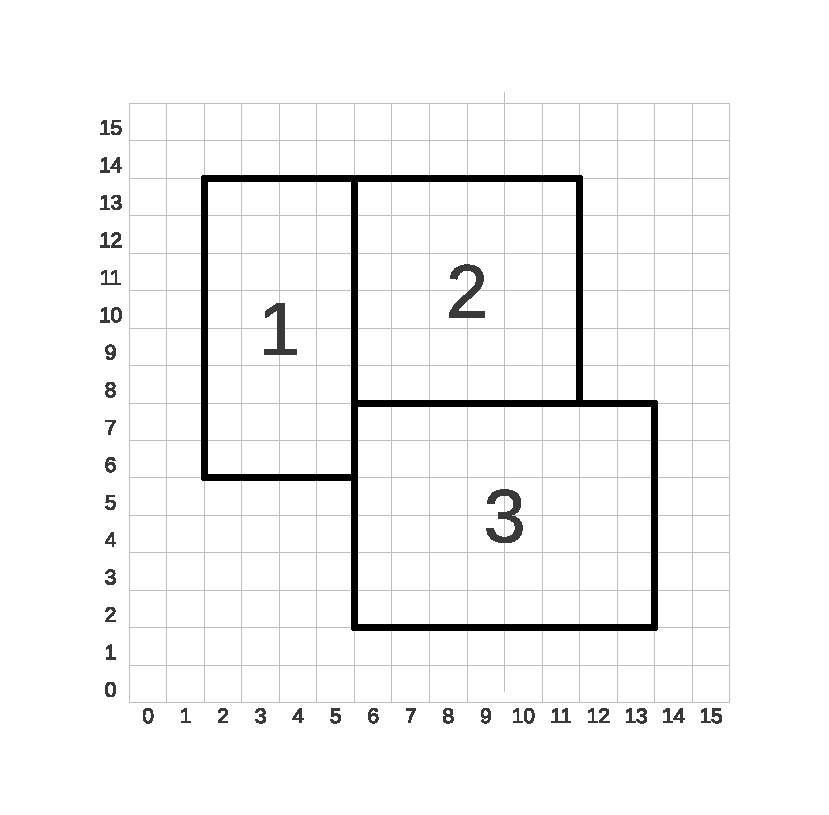
\includegraphics[width=4.0in]{./Introduction/index_grid2}
\caption{\label{fig:boxes} Three boxes that comprise a single level.
At this level of refinement, the domain is 16$\times$16 cells and
the global index space runs from 0 to 15 in each coordinate direction.
Note that these grids cannot be at the coarsest level,
since it would require that the grids span the problem domain.}
\end{figure}
%%%%%%%%%%%%%%%%%%%%%%%%%%%%%%%%%%%%%

\begin{itemize}
\item Example: For a simulation with 32 cells in each direction at the coarsest level,
the global index space for the coarsest level runs from 0 to 31 in each coordinate
direction.  Assuming refinement ratios of 2, the next finer level 
will have a global index space running from 
0 to 63 in each coordinate direction (corresponding to $64 \times
64$ zones if fully refined), and the next finer level will have a global index
space running from 0 to 127 in each coordinate direction
(corresponding to $128\times 128$ zones if fully refined).
\end{itemize}

\subsection{\BoxArray}

A \BoxArray\ is an array of \BoxType es.  The size of the array is the 
number of \BoxType es in the \BoxArray.  Suppose your problem domain
has lo indices (0,0) and hi indices (15,15), and you want to define
a \BoxArray\ to contain four $8\times 8$ boxes to cover the problem domain.
In Fortran90, you could do the following:
\begin{lstlisting}[backgroundcolor=\color{light-green}]
integer        :: lo(2), hi(2)
type(box)      :: bx(4)
type(boxarray) :: ba
lo(1) = 0
lo(2) = 0
hi(1) = 7
hi(2) = 7
bx(1) = make_box(lo,hi)
lo(1) = 8
lo(2) = 0
hi(1) = 15
hi(2) = 7
bx(2) = make_box(lo,hi)
lo(1) = 0
lo(2) = 8
hi(1) = 7
hi(2) = 15
bx(3) = make_box(lo,hi)
lo(1) = 8
lo(2) = 8
hi(1) = 15
hi(2) = 15
bx(4) = make_box(lo,hi)
call boxarray_build_v(ba,bx)
\end{lstlisting}
This is rather cumbersome, so instead we use other \BoxLib\ functions to
build the same \BoxArray:
\begin{lstlisting}[backgroundcolor=\color{light-green}]
type(boxarray) :: ba
integer        :: lo(2), hi(2)
type(box)      :: bx
lo(1:2) = 0
hi(1:2) = 15
bx = make_box(lo,hi)
call boxarray_build_bx(ba,bx)  ! the boxarray has one 16^2 box
call boxarray_maxsize(ba,8)    ! the boxarray has four 8^2 boxes
\end{lstlisting}
The analogous code in C++ is
\begin{lstlisting}[backgroundcolor=\color{light-blue}]
IntVect lo(0,0), hi(15,15);
Box bx(lo,hi);
BoxArray ba(bx);  // the BoxArray has one 16^2 box
ba.maxSize(8);    // the BoxArray has four 8^2 boxes
\end{lstlisting}

\subsection{\layout\ (Fortran90 Only)}

A \layout\ is a more intelligent \BoxArray, since it contains a \BoxArray\ as well
as the associated processor assignments, \BoxType\ connectivity, and many other
parallel constructs.  In the simplest case, if we have a \BoxArray\ {\tt ba} (obtained
from the example above), a 
\layout\ can be defined using:
\begin{lstlisting}[backgroundcolor=\color{light-green}]
type(layout) :: la
call layout_build_ba(la,ba)
\end{lstlisting}
In C++, the information that is contained in the Fortran90 \layout\ is part of
the \MultiFab\ class.

\subsection{\FArrayBox}

A \FArrayBox\ (or \Fab) is a ``Fortran array box'' that holds data.  It contains the
\BoxType\ that it is built on as well as a pointer to the data 
that can be sent to a Fortran routine.
In Fortran90, \Fab\ data is stored in a four-dimensional array,
{\tt (nx,ny,nz,nc)} in size, regardless of the dimensionality of the
problem.  Here {\tt nc} is the number of components, for instance
representing different fluid variables.  For 2D problems, {\tt nz=1}.\\

In \BoxLib, we don't usually deal with 
\Fab s alone, but rather through \MultiFab s, described next.

\section{The \MultiFab}
\MultiFab s are so important that we will give them their own section.
A \MultiFab\ is a collection of all the \Fab s at the same level of
refinement.
\begin{itemize}
\item In C++, a \MultiFab\ is defined using a \BoxArray,
number of components, and number of ghost cells that each \Fab\
will have.
\item In Fortran90, a \MultiFab\ is defined using a \layout,
number of components, and number of ghost cells that each \Fab\
will have.
\end{itemize}
A \MultiFab\ has a ``valid'' region that is defined by 
the \BoxArray or \layout.  Each \Fab\ in the \MultiFab\ is built large enough 
to hold valid data and ghost cell data, and thus the \BoxType\ associated with
each \Fab\ is a grown version of the corresponding \BoxType\ from the \BoxArray.
Thus, a \Fab\ has no concept 
of ghost cells, it merely has a single \BoxType\ that identifies it.\\

To build a \MultiFab, we require a \layout\ (in Fortran90) or a \BoxArray\ (in C++).
In Fortran90, using the \layout\ built above, we build a \MultiFab\ using:
\begin{lstlisting}[backgroundcolor=\color{light-green}]
type(multifab) :: data
call multifab_build(data,la,2,6) ! build the multifab with 2 components 
                                 ! and 6 ghost cells

...                              ! do fun stuff with the data

call multifab_destroy(data)      ! free up memory to prevent leaks
\end{lstlisting}
In C++, using the \BoxArray\ built above, you could either directly 
build a \MultiFab\ using:
\begin{lstlisting}[backgroundcolor=\color{light-blue}]
MultiFab data(ba,2,6);                     // build a MultiFab
\end{lstlisting}
or a pointer to a \MultiFab\ using:
\begin{lstlisting}[backgroundcolor=\color{light-blue}]
MultiFab* data = new MultiFab(ba,2,6);     // build pointer to MultiFab

...                                        // do fun stuff with the data

delete data;                               // need to free the memory
\end{lstlisting}

\subsection{Accessing \MultiFab\ Data}
Here is some sample Fortran90 code to access data within a \MultiFab:
\begin{lstlisting}[backgroundcolor=\color{light-green}]
integer                  :: i,dm,ng,nc,lo(2),hi(2)
type(multifab)           :: data
real(kind=dp_t), pointer :: dp(:,:,:,:)

...    ! build multifab ``data'' as described above

dm = data%dim   ! dm is dimensionality
ng = data%ng    ! ng is number of ghost cells
nc = data%nc    ! nc is number of components

! loop over the grids owned by this processor
do i=1,nfabs(data)
   dp => dataptr(data,i)          ! dp points to data inside fab
   lo = lwb(get_box(data,i))      ! get lo indices of box
   hi = upb(get_box(data,i))      ! get hi indices of box
   select case(dm)
   case (2)
      call work_on_data_2d(dp(:,:,1,:), ng, nc, lo, hi)
   case (3)
      call work_on_data_3d(dp(:,:,:,:), ng, nc, lo, hi)
    end select
end do

! fill periodic domain boundary and neighboring grid ghost cells
call multifab_fill_boundary(data)  

...

subroutine work_on_data_2d(data, ng, nc, lo, hi)

  integer          :: lo(2), hi(2), ng
  double precision :: data(lo(1)-ng:,lo(2)-ng:,:)

  ! local variables
  integer :: i,j,n

  do j=lo(2),hi(2)
     do i=lo(1),hi(1)
        do n=1,nc
           ! some silly function I made up
           data(i,j,n) = (i + j) * n
        end do
     end do
  end do

end subroutine work_on_data_2d
\end{lstlisting}

In C++:
\begin{lstlisting}[backgroundcolor=\color{light-blue}]
#if    defined(BL_FORT_USE_UPPERCASE)
#define FORT_WORK_ON_DATA            WORK_ON_DATA
#elif  defined(BL_FORT_USE_LOWERCASE)
#define FORT_WORK_ON_DATA            work_on_data
#elif  defined(BL_FORT_USE_UNDERSCORE)
#define FORT_WORK_ON_DATA            work_on_data_
#endif

extern "C"
{
    void FORT_WORK_ON_DATA (
        Real* data, const int* Ncomp, const int* ng,
        const int* lo, const int* hi);
}

int main()
{
  int Ncomp = 2, Nghost = 6;

  ...    // build pointer to MultiFab* ``data'' as described above
  
  // MFIter is a ``MultiFab Iterator'' that essentially
  // loops over grids
  for ( MFIter mfi(*data); mfi.isValid(); ++mfi )
  {
    const Box& bx = mfi.validbox();
    FORT_WORK_ON_DATA((*data)[mfi].dataPtr(),
                      &Nghost, &Ncomp, bx.loVect(), bx.hiVect());
  }
  // fill periodic domain boundary and neighboring grid ghost cells
  data->FillBoundary();
}
\end{lstlisting}
The {\tt FORT\_WORK\_ON\_DATA} calls a Fortran90 subroutine which is nearly
identical to the Fortran90 example given above.  The only difference is the subroutine
name cannot have the \_2d or \_3d in its name.  Thus, the 2d and 3d versions
are both named {\tt subroutine work\_on\_data}, and must be written in
different .f90 files, where the make system determines which version to compile
based on {\tt DIM}.\\

The {\tt multifab\_fill\_boundary} and {\tt FillBoundary} functions 
fill all ghost cells on periodic domain boundaries, as well as interior
ghost cells with values that can simply be copied from the valid region of a neighboring
grid at the same level of refinement.  For single-level problems that are periodic
in all directions, these functions fill all ghost cells.  We will discuss
non-periodic domain boundaries and fine grid ghost cells near coarse-fine interfaces
in Chapter \ref{Sec:Boundary Conditions}.

\subsection{Other \MultiFab\ Functions}
{\tt setVal} is a simple subroutine that sets the \MultiFab\ data to a particular value.
In Fortran90, use:
\begin{lstlisting}[backgroundcolor=\color{light-green}]
! set all variables to 0.0; ``all=.true.'' means set the ghost cells also
call setval(data,0.d0,all=.true.)
\end{lstlisting}
In C++, use:
\begin{lstlisting}[backgroundcolor=\color{light-blue}]
data->setVal(0.0);  // set all variables to 0.0, including ghost cells
\end{lstlisting}
{\tt copy} is a simple subroutine that copies data from one \MultiFab\ to another.
In Fortran90, use:
\begin{lstlisting}[backgroundcolor=\color{light-green}]
! copy components 1 and 2 from data_src into data_dest, 
! including the ghost cells. calling sequence is 
! (1) destination multifab, (2) first component of destination, 
! (3) source multifab, ! (4) first component of source, 
! (5) number of components, (6) ghost cells
call multifab_copy_c(data_dest,1,data_src,1,2,6)
\end{lstlisting}
In C++, use:
\begin{lstlisting}[backgroundcolor=\color{light-blue}]
// copy components 0 and 1 from data_src into data_dest, 
// including the ghost cells. calling sequence is 
// (1) destination multifab, (2) source multifab, 
// (3) first component of destination, (4) first component of source, 
// (5) number of components, (6) ghost cells
MultiFab::Copy(*data_dest,*data_src,0,0,2,6)
\end{lstlisting}
There are many other subroutines available for adding, subtracting, multiplying, etc.,
components of \MultiFab s, finding the min/max value, norms, number of cells, etc.
Refer to {\tt BoxLib/Src/F\_BaseLib/multifab\_f.f90} or 
{\tt BoxLib/Src/C\_BaseLib/MultiFab.H} for a complete listing.

\section{Simple Example - Fortran90}
We now provide a complete tutorial code that uses some concepts discussed above.
The code also writes plotfiles that can be viewed, and can be run in parallel if you
are working on a machine with MPI and/or OpenMP support.  The Fortran90 version of this 
example is contained in {\tt BoxLib/Tutorials/HeatEquation\_EX1\_F/}.\\

In this example, we advance the equation:
\begin{equation}
\frac{\partial\phi}{\partial t} = \nabla^2 \phi; \quad \phi(t=0) = 1 + e^{-100r^2},
\end{equation}
on a domain from [-1,1] in each spatial direction, where $r$ is the distance
to the point $(x,y,z) = (0.25,0.25,0.25)$.  Note that we are placing the
initial Gaussian profile slightly off-center.  This asymmetry will be important
in later sections when we examine the effects of non-periodic boundary conditions.
We will assume that $\Delta x = \Delta y = \Delta z$ and use a fixed
time step with $\Delta t = 0.9\Delta x^2$.  We begin with a simple 
single-level, forward Euler discretization, periodic boundary conditions,
and no refinement (i.e., only one level).\\

The basic time-advancement strategy uses the following temporal discretization:
\begin{equation}
\frac{\phi_{ij}^{n+1} - \phi_{ij}^n}{\Delta t} = \left[\nabla\cdot(\nabla\phi)\right]_{ij}.
\end{equation}
In the explicit case, we first compute $\nabla\phi$, at faces using:
\begin{equation}
(\nabla\phi)_{i+\myhalf,j} = \frac{\phi_{i+1,j}^n-\phi_{ij}^n}{\Delta x}.
\end{equation}
We will refer to these face-centered gradients as ``fluxes''.
Next, we compute the update by taking the divergence of these fluxes,
\begin{equation}
\left[\nabla\cdot(\nabla\phi)\right]_{ij} = \frac{(\nabla\phi)_{i+\myhalf,j}-(\nabla\phi)_{i-\myhalf,j}}{\Delta x} + \frac{(\nabla\phi)_{i,j+\myhalf}-(\nabla\phi)_{i,j-\myhalf}}{\Delta y}.
\end{equation}
We use a flux divergence formulation because it will enable a more natural 
extension to multiple levels of refinement, where we will be concerned with
conservation across levels.  Note that in this explicit case, since $\Delta x = \Delta y$, 
the Laplacian reduces to the standard five point stencil in two dimensions
(seven point stencil in three dimensions).\\

Since the fluxes live on faces, we need face-centered \MultiFab s, i.e.,
\MultiFab s that are nodal in one spatial direction.  In {\tt advance.f90},
we build them as follows:
\begin{lstlisting}[backgroundcolor=\color{light-green}]
! an array of multifabs; one for each direction
type(multifab) :: flux(phi%dim) 

! build the flux(:) multifabs
do i=1,dm
   ! flux(i) has 1 component, 0 ghost cells, and is nodal in direction i
   call multifab_build_edge(flux(i),phi%la,1,0,i)
end do
\end{lstlisting}

In the problem directory, you will see the following files:
\begin{itemize}
\item {\tt GNUmakefile}

This contains compiler settings and directories required by the make system to build the code.

  \begin{itemize}

    \item {\tt BOXLIB\_HOME}

    Change this to point to the \BoxLib\ home directory.  Alternatively, you can define {\tt BOXLIB\_HOME}
    as an environment variable on your system.

    \item {\tt NDEBUG} ('{\tt t}' or '{\tt <blank>}') for TRUE or FALSE
      
    ``not debug'' (we know, confusing).  If '{\tt t}', modifies compiler flags to build a 
    more optimized version of the code.  The program will run faster, but have fewer 
    runtime error checks.

    \item {\tt MPI} ('{\tt t}' or '{\tt <blank>}')

    Indicate whether you want your executable to be MPI-compatible.  MPI must be installed on your
    machine in order to use this, and you must modify some of the make scripts, as will be 
    discussed later.

    \item {\tt OMP} ('{\tt t}' or '{\tt <blank>}')

    Turns on OpenMP compiler flags to compile in any OpenMP directives in the code.
    We will discuss OpenMP further in Section \ref{Sec:OpenMP}.

    \item {\tt PROF} ('{\tt t}' or '{\tt <blank>}')

    Turns on timer compilation flags.  Timers are useful for optimizing your code since they tell you 
    what subroutines are taking the most time and require more optimization.  Note that you still have 
    to write timers into your code.  We will discuss the implementation of timers in Section \ref{Sec:Timers}.

    \item {\tt COMP} ('{\tt gfortran}, {\tt Intel}, $\ldots$)'

    The Fortran compiler.  Supported options include {\tt gfortran}, {\tt Intel}, 
    {\tt PathScale}, {\tt PGI}, and {\tt Cray}.  The {\tt gfortran} compiler seems to be 
    bug-free on all systems we've run on, so stick with this unless you have good reason to 
    change.  {\tt Intel} after version 9 seems flaky.  {\tt PathScale} (available 
    at OLCF and NERSC) seems to work as long as you don't turn the optimization flags 
    too high, and seems to run the fastest if you can actually get it to work.  
    {\tt Cray} seems to give similar performance as {\tt PathScale} (perhaps
    because Cray bought out PathScale recently).  {\tt PGI} (available at OLCF and NERSC) 
    seems to work fine, but is slower than the others.

    \item {\tt MKVERBOSE} ('{\tt t}' or '{\tt <blank>}')

    Verbosity of compile-time output.

  \end{itemize}

\item {\tt GPackage.mak}

List of local files needed to be included in the build.  The {\tt GNUmakefile} points to this.

\item {\tt main.f90}, {\tt init\_phi.f90}, {\tt advance.f90}, {\tt write\_plotfile.f90}

Source code that is not within the {\tt BoxLib/Src/} tree.  Note that 
if a file that exists in the
{\tt BoxLib/Src/} tree also exists in the local directory, the local copy takes precedence
as long as the {\tt GNUmakefile} lists your local directory as a {\tt VPATH\_LOCATIONS} 
before the \BoxLib\ source code directory, {\tt BoxLib/Src/F\_BaseLib}.

\item {\tt inputs\_2d}, {\tt inputs\_3d}

Input files to customize the simulation parameters.

\end{itemize}

To build the code, edit the {\tt GNUmakefile} and simply type ``{\tt make}''.  An 
exectubale will appear that has some indication (but not complete)
about what setting you used in the {\tt GNUmakefile}.  To run the code on a single processor,
simply type, for example (terminal commands and non-source code files are shaded in red),
\begin{lstlisting}[backgroundcolor=\color{light-red}]
./main.Linux.gfortran.exe inputs_2d
\end{lstlisting}
The program will complete and there will be a series of plotfiles, e.g., {\tt plt00000}, 
{\tt plt00100}, etc., in the run directory.  You can visualize the data 
and make animations using {\tt VisIt} (available at {\tt https://wci.llnl.gov/codes/visit/});
refer to Section \ref{Sec:VisIt}.

\section{Simple Example - C++}
The C++ version of this example is contained in {\tt BoxLib/Tutorials/HeatEquation\_EX1\_C/}.

\begin{itemize}
\item {\tt GNUmakefile}

This contains compiler settings and directories required by the make system to build the code.

  \begin{itemize}

    \item {\tt BOXLIB\_HOME}

    Change this to point to the \BoxLib\ home directory.  Alternatively, you can define {\tt BOXLIB\_HOME}
    as an environment variables on your system.

    \item {\tt DEBUG} ('{\tt TRUE}' or '{\tt FALSE}')
      
    Debug mode.  If 'FALSE', modifies compiler flags to build a more optimized version of the code.
    The program will run faster, but have fewer runtime error checks.

    \item {\tt USE\_MPI} ('{\tt TRUE}' or '{\tt FALSE}')

    Indicate whether you want your executable to be MPI-compatible.  MPI must be installed on your
    machine in order to use this, and you must modify some of the make scripts, as will be 
    discussed later.

    \item {\tt USE\_OMP} ('{\tt TRUE}' or '{\tt FALSE}')
    
    Turns on OpenMP compiler flags to compile in any OpenMP directives in the code.
    We will discuss OpenMP further in Chapter \ref{Sec:OpenMP}.

    \item {\tt PROFILE} ('{\tt TRUE}' or '{\tt FALSE}')

    Turns on timer compilation flags.  Timers are useful for optimizing your code since they tell you 
    what subroutines are taking the most time and require more optimization.  Note that you still have 
    to write timers into your code.  We will discuss the implementation of timers in Chapter \ref{Sec:Timers}.

    \item {\tt COMP} ('{\tt g++}, {\tt Intel}, $\ldots$)'

    The C++ compiler.  Supported options include {\tt g++}, {\tt Intel}, {\tt PathScale}, 
    {\tt PGI}, and {\tt Cray}.  See compiler notes above.

    \item {\tt FCOMP} ('{\tt gfortran}, {\tt Intel}, $\ldots$)'

    The Fortran compiler.  See compiler notes above.

    \item {\tt DIM} ('1', '2', or '3')

    Dimensionality of the problem.  Unlike Fortran90, you need to set this in the C++ version.

    \item {\tt PRECISION} ('{\tt DOUBLE}' or '{\tt FLOAT}')

    Precision of real numbers.  You can use {\tt FLOAT} for single-precision real numbers to save memory.

    \item {\tt EBASE} ('{\tt main}', $\ldots$)

    The executable string will begin with this.

  \end{itemize}

\item {\tt Make.package}

List of local files needed to be included in the build.  The {\tt GNUmakefile} points to this.

\item {\tt main.f90}, {\tt writePlotFile.cpp}, {\tt writePlotFile.H}, {\tt init\_phi\_2d.f90},
      {\tt init\_phi\_3d.f90}, {\tt advance\_2d.f90}, {\tt advance\_3d.f90}

Source code that is not within the {\tt BoxLib/Src/} tree.  Note that if a file that 
exists in the
{\tt BoxLib/Src/} tree also exists in the local directory, the local copy takes precedence
as long as the {\tt GNUmakefile} lists your local directory in the {\tt include} line before
before the \BoxLib\ source code directories.

\item {\tt inputs\_2d}, {\tt inputs\_3d}

Input files to customize the simulation parameters.

\end{itemize}

To build the code, simply type ``{\tt make}''.  An exectubale will appear that has some indication (but not complete)
about what setting you used in the {\tt GNUmakefile}.  To run the code on one processor, simply type, for example,
\begin{lstlisting}[backgroundcolor=\color{light-red}]
./main2d.Linux.g++.gfortran.ex inputs_2d
\end{lstlisting}
The program will complete and there will be a series of plotfiles, e.g., {\tt plt00000}, 
{\tt plt00100}, etc., in the run directory.  You can visualize the data 
and make animations using {\tt VisIt} (available at {\tt https://wci.llnl.gov/codes/visit/});
refer to Section \ref{Sec:VisIt}.

\section{Visualization Using {\tt VisIt}}\label{Sec:VisIt}
First, download and install {\tt VisIt} from {\tt https://wci.llnl.gov/codes/visit/}.
To open a single plotfile, run {\tt VisIt}, then select ``File'' $\rightarrow$ ``Open file ...'',
then select the {\tt Header} file associated the the plotfile of interest (e.g., {\tt plt00000/Header}).
Assuming you ran the simulation in 2D, here are instructions for making a simple plot:
\begin{itemize}
\item To view the data, select ``Add'' $\rightarrow$ ``Pseudocolor'' $\rightarrow$ ``phi'', and then select
``Draw''.
\item To view the grid structure (not particularly interesting yet, but when we add AMR it will be), select
`` $\rightarrow$ ``subset'' $\rightarrow$ ``levels''.  Then double-click the text ``Subset - levels'',
enable the ``Wireframe'' option, select ``Apply'', select ``Dismiss'', and then select ``Draw''.
\item To save the image, select ``File'' $\rightarrow$ ``Set save options'', then customize the image format
to your liking, then click ``Save''.
\end{itemize}
Your image should look similar to the left side of Figure \ref{Fig:VisIt}.\\
\begin{figure}[tb]
\centering
\includegraphics[width=3.1in]{./GettingStarted/VisIt_2D}
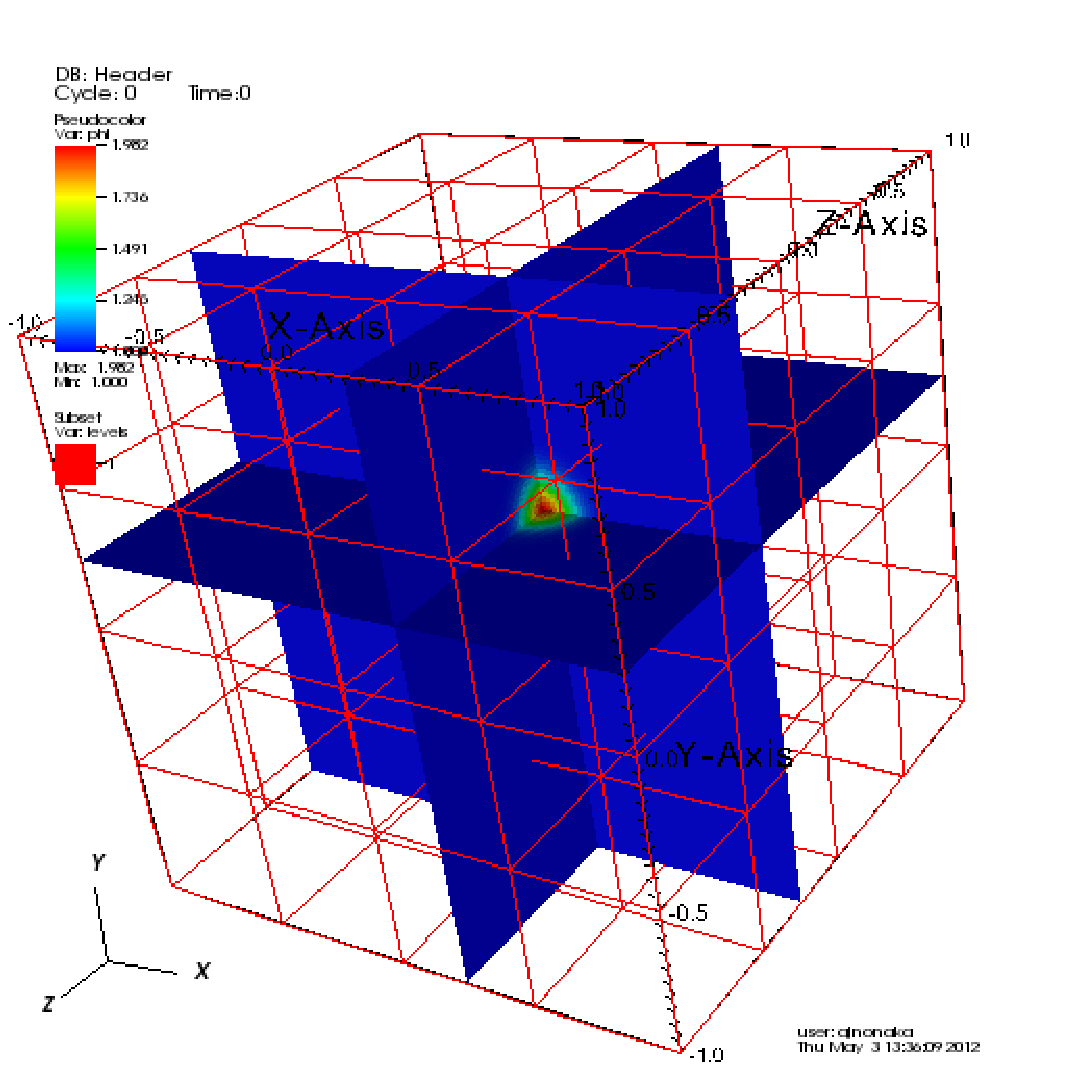
\includegraphics[width=3.1in]{./GettingStarted/VisIt_3D}
\caption{(Left) 2D image generated with VisIt.  (Right) 3D image generated with VisIt.}
\label{Fig:VisIt}
\end{figure}

In 3D, you must apply the ``Operators'' $\rightarrow$ ``Slicing'' $\rightarrow$ ``ThreeSlice'', with the 
``ThreeSlice operator attribute'' set to x=0.25, y=0.25, and z=0.25.  You can left-click and drag
over the image to rotate the image to generate something similar to right side of Figure \ref{Fig:VisIt}.\\

To make a movie, you must first create a text file named {\tt movie.visit} with a list of the {\tt Header} 
files for the individual frames.  This can most easily be done using the command:
\begin{lstlisting}[backgroundcolor=\color{light-red}].
~/BoxLib/Tutorials/HeatEquation_EX1_F> ls -1 plt*/Header | tee movie.visit
plt00000/Header
plt01000/Header
plt02000/Header
plt03000/Header
plt04000/Header
plt05000/Header
plt06000/Header
plt07000/Header
plt08000/Header
plt09000/Header
plt10000/Header
\end{lstlisting}
The next step is to run {\tt VisIt}, select ``File'' $\rightarrow$ ``Open file ...'',
then select {\tt movie.visit}.  Create an image to your liking and press the ``play'' button
on the VCR-like control panel to preview all the frames.  To save the movie, choose
``File'' $\rightarrow$ ``Save movie ...'', and follow the on-screen instructions.

\section{Running in Parallel with MPI}
We will now demonstrate how to run the example in {\tt BoxLib/Tutorials/HeatEquation\_EX1\_F/}
using MPI parallelism.  To run in parallel using C++ \BoxLib\ is analogous.
On your local machine, if you have MPI installed, you must first configure
{\tt BoxLib/Tools/F\_mk/GMakeMPI.mak} and {\tt BoxLib/Tools/C\_mk/Make.mpi}
to your MPI installation.  Then, you 
can simply build the executable as describe before, but with {\tt MPI=t} 
in the {\tt GNUmakefile}.  Alternatively, you can override the settings in 
{\tt GNUmakefile} at the command line using, e.g., ``{\tt make MPI=t}''.  
An executable named {\tt main.Linux.gfortran.mpi.exe} will be built.
Then you can run the program in parallel using, e.g.,
\begin{lstlisting}[backgroundcolor=\color{light-red}].
mpiexec -n 4 main.Linux.gfortran.mpi.ex inputs_2d
\end{lstlisting}

To run in parallel on the hopper machine at NERSC, first copy the \BoxLib\ source code
into your home directory on hopper and go to the {\tt HeatEquation\_EX1\_F/} directory.
The default programming environment uses the {\tt PGI} compilers, so we will switch to the
{\tt gnu} programming environment to make {\tt g++} and {\tt gfortran} available
using the command:
\begin{lstlisting}[backgroundcolor=\color{light-red}].
module swap PrgEnv-pgi PrgEnv-gnu
\end{lstlisting}
Next, in {\tt GNUmakefile}, set {\tt MPI=t}, and then type ``{\tt make}''
(or alternatively, type ``{\tt make MPI=t}'').
An executable named {\tt main2d.Linux.g++.gfortran.mpi.exe} will be built.
You cannot submit jobs in your home directory, so change to a scratch space
(``{\tt cd \$SCRATCH}'' will typically do), and copy the executable and
{\tt inputs\_2d} into this directory.  Then you need to create a job script,
e.g., "{\tt hopper.run}", that has contents (for tcsh):
\lstinputlisting[backgroundcolor=\color{light-red}]{./GettingStarted/hopper.run}
Note that ``mppwidth'' and ``-n'' both indicate the number of cores you are requesting.
To run, simply type ``{\tt qsub hopper.run}''.  You can monitor the status of your job
using ``{\tt qstat -u <username>}'' and view your position in the queue 
using ``{\tt showq}''.

\section{Running in Parallel with MPI/OpenMP (3D ONLY)}\label{Sec:OpenMP}
Both the C++ and Fortran versions of this tutorial also support hybrid MPI/OpenMP parallelism for {\bf three-dimensional problems only}.
You may add OMP parallelism to two-dimensional work loops, but be advised that subroutines within the \BoxLib~ infrastructure 
are not threaded for two-dimensional problems.
To ``thread'' the code, we have simply added OpenMP directives (using the {\tt !\$omp parallel do} 
construct) to any i/j/k loops we were interested in threading.  For example, in {\tt init\_phi.f90}:
\begin{lstlisting}[backgroundcolor=\color{light-green}]
!$omp parallel do private(i,j,k,x,y,z,r2)
do k=lo(3),hi(3)
   z = prob_lo(3) + (dble(k)+0.5d0) * dx
   do j=lo(2),hi(2)
      y = prob_lo(2) + (dble(j)+0.5d0) * dx
      do i=lo(1),hi(1)
         x = prob_lo(1) + (dble(i)+0.5d0) * dx

         r2 = ((x-0.25d0)**2 + (y-0.25d0)**2 + (z-0.25d0)**2) / 0.01d0
         phi(i,j,k) = 1.d0 + exp(-r2)
 
      end do
   end do
end do
!$omp end parallel do
\end{lstlisting}
This User's Guide is not a manual on OpenMP, so simply note that this particular 
construct tells each thread to work on different values of {\tt k}, with each 
thread getting its own local copy of {\tt i}, {\tt j}, {\tt x}, {\tt y}, {\tt z}, and {\tt r2}.\\

Finally, to tell the compiler that we would like to run with OpenMP, we make sure to
set {\tt OMP=t} (in Fortran) or {\tt USE\_OMP=TURE} (in C++) in the {\tt GNUmakefile}.
Otherwise, all OpenMP directive are
simply ignored.  Note that at runtime you must have set the 
{\tt OMP\_NUM\_THREADS} environment variable properly in order for threads to work.
Also, note that you can enable/disable MPI independently from the OMP flag.  Finally,
here is a sample hopper script (tcsh) for a hybrid MPI/OpenMP job:
\lstinputlisting[backgroundcolor=\color{light-red}]{./F_AdvancedTopics/hopper_omp.run}
\begin{itemize}
\item ``mppwidth'': how many total cores requested
\item ``-n'': total number of MPI tasks
\item ``-N'': number of MPI tasks per hopper node
\item ``-S'': number of MPI tasks per NUMA node
\item ``-ss'': demands strict memory containment per NUMA node
\item ``-d'': number of OpenMP threads per MPI task
\end{itemize}


\chapter{Building AMReX}\label{Chap:BuildingAMReX}

In this chapter, we discuss \amrex's build systems.  There are three
ways to use \amrex.  The approach used by \amrex\ developers uses GNU
Make.  There is no installation step in this approach.  Application
codes adopt \amrex's build system and compile \amrex\ while compiling
their own codes.  This will be discussed in more detail in
Section~\ref{sec:build:make}.  The second approach is to build \amrex\
into a library and install it (Section~\ref{sec:build:lib}).  Then an
application code uses its own build system and links \amrex\ as an
external library.  \amrex\ can also be built with Cmake
(Section~\ref{sec:build:cmake}).

\section{Building with GNU Make}
\label{sec:build:make}

In this build approach, you write your own make files defining a
number of variables and rules.  Then you invoke {\tt make} to start
the building process.  This will result in an executable upon
successful completion.  The temporary files generated in the building
process are stored in a temporary directory named {\tt
  tmp\_build\_dir}.

\subsection{Dissecting a Simple Make File}

An example of building with GNU Make can be found in {\tt
  amrex/Tutorials/Basic/HelloWorld\_C}.  Table~\ref{tab:makevarimp}
shows a list of important variables.
\begin{table}[t]
  \centering
  \begin{tabular}{lcc}
    Variable & Value & Default \\
    \hline
    {\tt AMREX\_HOME} & Path to amrex & environment \\
    {\tt COMP} & {\tt gnu}, {\tt cray}, {\tt ibm}, {\tt intel}, {\tt llvm}, or {\tt pgi} & none \\
    {\tt DEBUG} & {\tt TRUE} or {\tt FALSE} & {\tt TRUE} \\
    {\tt DIM} & 1 or 2 or 3 & none \\
    {\tt USE\_MPI} & {\tt TRUE} or {\tt FALSE} & {\tt FALSE} \\
    {\tt USE\_OMP} & {\tt TRUE} or {\tt FALSE} & {\tt FALSE} \\
    \hline
  \end{tabular}
  \caption{\label{tab:makevarimp} Important make variables}
\end{table}

At the beginning of {\tt
  amrex/Tutorials/Basic/HelloWorld\_C/GNUmakefile}, {\tt AMREX\_HOME}
is set to the path to the top directory of \amrex.  Note that in the
example {\tt ?=} is a conditional variable assignment operator that
only has an effect if {\tt AMREX\_HOME} has not been defined
(including in the environment).  One can also set {\tt AMREX\_HOME} 
as an environment variable.  For example in bash, 
one can set {\tt export AMREX\_HOME=/path/to/amrex}; in tcsh one can set
{\tt setenv AMREX\_HOME /path/to/amrex}.

One must set the {\tt COMP} variable to choose a compiler.  Currently
the list of supported compilers includes {\tt gnu}, {\tt cray}, {\tt
  ibm}, {\tt intel}, {\tt llvm}, and {\tt pgi}.  One must also set the
{\tt DIM} variable to either 1, 2, or 3, depending on the
dimensionality of the problem.

Variables {\tt DEBUG}, {\tt USE\_MPI} and {\tt USE\_OMP} are optional
with default set to {\tt TRUE}, {\tt FALSE} and {\tt FALSE},
respectively.  The meaning of these variables should be obvious.  
When {\tt DEBUG = TRUE}, aggressive compiler optimization flags are turned
off and assertions in \amrex\ source code are turned on.  For
production runs, {\tt DEBUG} should be set to {\tt FALSE}.

After defining these make variables, a number of files, {\tt
  Make.defs}, {\tt Make.package} and {\tt Make.rules}, are included in
{\tt GNUmakefile}.  \amrex\-based applications do not need to include
all directories in \amrex; an application which does not use particles,
for example, does not need to include files from the {\tt Particle}
directory in its build.
In this simple example, we only need to include {\tt
  \$(AMREX\_HOME)/Src/Base/Make.package}.  An application code also
has its own {\tt Make.package} file (e.g., {\tt ./Make.package} in
this example) to append source files to the build system using
operator {\tt +=}.  Variables for various source files are shown
below.
\begin{quote}
\begin{description}
\item [{CEXE\_sources}] \cpp\ source files.  Note that \cpp\
  source files are assumed to have a {\tt .cpp} extension.
\item [{CEXE\_headers}] \cpp\ headers with {\tt .h} or {\tt .H} extension.
\item [{cEXE\_sources}] C source files with {\tt .c} extension.
\item [{cEXE\_headers}] C headers with {\tt .h} extension.
\item [{f90EXE\_sources}] Free format Fortran source with {\tt
    .f90} extension.
\item [{F90EXE\_sources}] Free format Fortran source with {\tt
    .F90} extension.  Note that these Fortran files will go through
  preprocessing.
\end{description}
\end{quote}
In this simple example, the extra source file, {\tt main.cpp} is in
the current directory that is already in the build system's search
path.  If this example has files in a subdirectory (e.g., {\tt
  mysrcdir}), you will then need to add the following to {\tt
  Make.package}. 
\begin{verbatim}
    VPATH_LOCATIONS += mysrcdir
    INCLUDE_LOCATIONS += mysrcdir
\end{verbatim}
Here {\tt VPATH\_LOCATIONS} and {\tt INCLUDE\_LOCATIONS} are the search
path for source and header files, respectively.

\subsection{Tweaking Make System}

The GNU Make build system is located at {\tt amrex/Tools/GNUMake}.
You can read {\tt README.md} and the make files there for more
information.  Here we will give a brief overview.

Besides building executable, other common make commands include:
\begin{quote}
\begin{description}
  \item[make clean] This removes the executable, {\tt .o} files, and
    the temporarily generated files.  Note that one can add additional
    targets to this rule by using the double colon (::)
  \item[make realclean] This removes all files generated by make.
  \item[make help] This shows the rules for compilation.
  \item[make print-xxx] This shows the value of variable {\tt xxx}.  This is
    very useful for debugging and tweaking the make system.
\end{description}
\end{quote}

Compiler flags are set in {\tt amrex/Tools/GNUMake/comps/}.  Note that
variables like {\tt CC} and {\tt CFLAGS} are reset in that directory
and their values in environment variables are disregarded. Site
specific setups (e.g., MPI installation) are in {\tt
  amrex/Tools/GNUMake/sites/}, which includes a generic setup in {\tt
  Make.unknown}.  You can override the setup by having your own {\tt
  sites/Make.\$(host\_name)} file, where variable {\tt host\_name} is your
host name in the make system and can be found via {\tt make
  print-host\_name}.  You can also have a {\tt
  amrex/Tools/GNUMake/Make.local} file to override various variables.
See {\tt amrex/Tools/GNUMake/Make.local.template} for an example.

\section{Building {\tt libamrex}}
\label{sec:build:lib}

If an application code already has its own elaborated build system and
wants to use \amrex\ as an external library, this might be your
choice.  In this approach, one runs {\tt ./configure}, followed by
{\tt make} and {\tt make install}.  In the top \amrex\ directory, one
can run {\tt ./configure -h} to show the various options for the {\tt
  configure} script.  This approach is built on the \amrex\ GNU Make
system.  Thus Section~\ref{sec:build:make} is recommended if any fine
tuning is needed.

\section{Building with CMake}
\label{sec:build:cmake}

An alternative to the approach described in Section~\ref{sec:build:lib}
is to install \amrex\ as an external library by using the CMake build system.
A CMake build is a two-steps process. First {\tt cmake} is invoked to create 
configuration files and makefiles in a chosen directory ({\tt builddir}). 
This is roughly equivalent to running  {\tt ./configure} (see Section
~\ref{sec:build:lib}). Next, the actual build and installation are performed
by issuing {\tt make install} from within {\tt builddir}. This will install
the library files in a chosen installation directory ({\tt installdir}).
The CMake build process is summarized as follow:
\begin{verbatim}
mkdir /path/to/builddir
cd    /path/to/builddir
cmake [options] -DCMAKE_INSTALL_PREFIX:PATH=<path/to/installdir>  /path/to/amrex 
make install
\end{verbatim} 
In the above snippet, {\tt [options]} indicates one or more options for the customization
of the build, as described in Subsection~\ref{sec:build:cmake:options}. 
Although the \amrex\ source could be used as build directory, we advise against doing so.
After the installation is complete, {\tt builddir} can be removed.
\subsection{Customization options}
\label{sec:build:cmake:options}
\amrex\ configuration settings may be specified on the command line with the {\tt -D} option.
For example one can enable OpenMP support as follows:
\begin{verbatim}
cmake -DENABLE_OMP=1 -DCMAKE_INSTALL_PREFIX:PATH=<path/to/installdir>  /path/to/amrex 
\end{verbatim} 
The list of available option is reported in Table~\ref{tab:cmakevar}.
\begin{table}[h!]
  \centering
  \begin{tabular}{llcc}
    Option name & Description & Default Value & Possible values  \\
    \hline
    {\tt CMAKE\_BUILD\_TYPE} & Type of \amrex\ build & Debug & Debug,Release \\    
    {\tt BL\_SPACEDIM} & Dimension of \amrex\ build & 3 & 2,3 \\
    {\tt ENABLE\_DP} & Enable double precision & 1 & 0,1 \\
    {\tt ENABLE\_MPI} & Enable build with MPI & 1 & 0,1 \\
    {\tt ENABLE\_OMP} & Enable build with OpenMP & 0 & 0,1 \\
    {\tt ENABLE\_PARTICLES} & Include particle classes in build & 0  & 0,1 \\
    {\tt ENABLE\_DP\_PARTICLES} & Enable double precision for particle classes & 1 & 0,1 \\    
    {\tt ENABLE\_PROFILING} &  Include profiling info in build & 0  & 0,1 \\
    {\tt ENABLE\_TINY\_PROFILING} &  Include tiny-profiling info in build & 0  & 0,1 \\
    {\tt ENABLE\_BACKTRACE} & Include backtrace info in  build & 1  & 0,1 \\
    {\tt AMREX\_FFLAGS\_OVERRIDES} &  User-defined Fortran flags & empty  & user-defined \\
    {\tt AMREX\_CXXFLAGS\_OVERRIDES} &  User-defined C++ flags & empty  & user-defined \\
    \hline
  \end{tabular}
  \caption{\label{tab:cmakevar} Variables for the customization of \amrex\ build with CMake}
\end{table}





\chapter{The Basics}\label{Chap:Basics}
In this chapter, we present the basics of \amrex.  The implementation
source codes are in {\tt amrex/Src/Base/}.  Note that \amrex\ classes
and functions are in namespace {\tt amrex}.  For clarity, we usually
drop {\tt amrex::} in the example codes here.  It is also assumed that
headers have been properly {\tt include}d.  We recommend you study
tutorials at {\tt amrex/Tutorials/Basic/} while reading this chapter.
After reading this chapter, one should be able to develop single-level
parallel codes using \amrex.  It should also be noted that this is not
a comprehensive reference manual.

\section{Dimensionality}
\label{sec:basics:dim}

As we have mentioned in Chapter~\ref{Chap:BuildingAMReX}, the
dimensionality of \amrex\ must be set at compile time.  A macro, {\tt
  AMREX\_SPACEDIM}, is defined to be the number of spatial
dimensions.  C++ codes can also use the {\tt amrex::SpaceDim}
variable.  Fortran codes can use either the macro and preprocessing or
do 
\begin{verbatim}
    use amrex_fort_module, only : amrex_spacedim
\end{verbatim}
The coordinate directions are zero based. \MarginPar{Not in Fortran}

\section{Array}

{\tt Array} class is derived from {\tt std::vector}.  The only
difference between {\tt Array} and {\tt std::vector} is that {\tt
  Array::operator[]} provides bound checking when compiled with {\tt
  DEBUG=TRUE}. 

\section{Real}

\amrex\ can be compiled to use either double precision (which is the
default) or single precision.  {\tt amrex::Real} is {\tt typedef}'d to
either {\tt double} or {\tt float}.  C codes can use {\tt
  amrex\_real}.  The data type is accessible in Fortran codes via
\begin{verbatim}
    use amrex_fort_module, only : amrex_real
\end{verbatim}

\section{ParallelDescriptor}

\amrex\ users do not need to use MPI directly.  Parallel communication
is often handled by the data abstraction classes (e.g., {\tt
  MultiFab}; Section~\ref{sec:basics:multifab}).  In addition, \amrex\
has provided {\tt namespace ParallelDesriptor}.  The frequently used
functions are 
\begin{lstlisting}[language=cpp]
 int myproc = ParallelDescriptor::MyProc();  // Return the rank
 
 int nprocs = ParallelDescriptor::NProcs();  // Return the number of processes
 
 if (ParallelDescriptor::IOProcessor()) { 
     // Only the I/O process executes this
 }
 
 int ioproc = ParallelDescriptor::IOProcessorNumber();  // I/O rank
 
 ParallelDescriptor::Barrier();
 
 // Broadcast 100 ints from the I/O Processor
 Array<int> a(100);
 ParallelDescriptor::Bcast(a.data(), a.size(),
                     ParallelDescriptor::IOProcessorNumber())
 
 // See AMReX_ParallelDescriptor.H for many other Reduce functions 
 ParallelDescriptor::ReduceRealSum(x);
\end{lstlisting}

\section{Print}
\label{sec:basics:print}

\amrex\ provides classes for printing messages to standard output or
any \cpp\ {\tt ostream}.  The main reason one should use them instead
of {\tt std::cout} is that messages from multiple processes or
threads do not get mixed up.  Below are some examples.
\begin{lstlisting}[language=cpp]
 Print() <<  "x = " << x << "\n"; // Print on I/O processor
 
 Real pi = std::atan(1.0)*4.0;
 // Print on rank 3 with precision of 17 digits
 // SetPrecision does not modify cout's floating-point decimal precision setting.
 Print(3).SetPrecision(17) << pi << "\n";

 int oldprec = std::cout.precision(10);
 Print() << pi << "\n";  // Print with 10 digits
 
 AllPrint() << "Every process prints\n";  // Print on every process
 
 std::ofstream ofs("my.txt", std::ofstream::out);
 Print(ofs) << "Print to a file" << std::endl;
 ofs.close();
\end{lstlisting}

\section{ParmParse}

{\tt ParmParse} is a class providing a database for the storage and
retrieval of command-line and input-file arguments.  When {\tt
  amrex::Initialize()} is called, the first command-line argument
after the executable name (if there is one and it does not contain
character {\tt =}) is taken to be the inputs file, and the contents in
the file are used to initialized the {\tt ParmParse} database.  The
rest of the command-line arguments are also parsed by {\tt ParmParse}.
The format of the inputs file is a series of definitions in the form
of {\tt prefix.name = value value ...}.  For each line, texts after a
{\tt \#} are comments.  Here is an example inputs file.
\begin{verbatim}
nsteps    = 100               # integer
nsteps    = 1000              # nsteps appears a second time
dt        = 0.03              # floating point number
ncells    = 128 64 32         # a list of 3 ints
xrange    = -0.5 0.5          # a list of 2 reals
title     = "Three Kingdoms"  # a string
hydro.cfl = 0.8               # with prefix, hydro 
\end{verbatim}
The following code shows how to use {\tt ParmParse} to get the values.
\begin{lstlisting}[language=cpp]
 ParmParse pp;
 
 int nsteps = 0;
 pp.query("nsteps", nsteps);
 amrex::Print() << nsteps << "\n";  // 1000
 
 Real dt;
 pp.get("dt", dt);  // runtime error if dt is not in inputs
 
 Array<int> numcells;
 // A different name say 'numcells' can be used
 pp.getarr("ncells", numcells);
 amrex::Print() << numcells.size() << "\n";  // 3
 
 Array<Real> xr {-1.0, 1.0};
 if (!queryarr("xrange", xr)) {
     amrex::Print() << "Cannot find xrange in inputs, "
                    << "so the default {-1.0,1.0} will be used\n";
 }
 
 std::string title;
 query("title", title);  // query string
 
 ParmParse pph("hydro");  // with prefix 'hydro'
 Real cfl;
 pph.get("cfl", cfl);    // get parameter with prefix
\end{lstlisting}
Note that when there are multiple definitions for a parameter {\tt
  ParamParse} by default returns the last one.  The difference between
{\tt query} and {\tt get} should also be noted.  It is a runtime error
if {\tt get} fails to get the value, whereas {\tt query} returns an
error code without generating a runtime error that will abort the run.
If it is sometimes convenient to override parameters with command-line
arguments without modifying the inputs file.  The command-line
arguments after the inputs file are added later to the database and
are therefore used be default.  For example, one can run with
\begin{verbatim}
    myexecutable myinputsfile ncells="64 32 16" hydro.cfl=0.9
\end{verbatim}
to change the value of {\tt ncells} and {\tt hydro.cfl}.

\section{Box, IntVect and IndexType}
\label{sec:basics:box}

In \amrex, the computational domain (on each AMR level) is decomposed
into a union of rectangular domains.  {\tt Box} is the data
structure for representing such rectangular domains in indexing space.
{\tt Box} is a dimension dependent class.  It has lower and upper
corners (represented by {\tt IntVect} and an index type
(represented by {\tt IndexType}).  There are no floating-point data in
the object.

\subsection{IntVect}

{\idxamrex{IntVect}} is a dimension dependent class representing an
integer vector in {\idxamrex{AMREX\_SPACEDIM}}-dimensional space.  An
{\tt IntVect} can be constructed as follows,
\begin{lstlisting}[language=cpp]
 IntVect iv(AMREX_D_DECL(19, 0, 5));
\end{lstlisting}
Here {\tt AMREX\_D\_DECL} is a macro that expands {\tt
  AMREX\_D\_DECL(19,0,5)} to either {\tt 19} or {\tt 19,0} or {\tt
  19,0,5} depending on the number of dimensions.  The data can be
accessed via {\tt operator[]}, and the internal data pointer can be
returned by function {\tt getVect}.  For example
\begin{lstlisting}[language=cpp]
 for (int idim = 0; idim < AMREX_SPACEDIM; ++idim) {
     amrex::Print() << "iv[" << idim << "] = " << iv[idim] << "\n";
 }
 const int * p = iv.getVect();  // This can be passed to Fortran/C as an array
\end{lstlisting}

The class has a static function {\tt TheZeroVector()} returning the
zero vector, {\tt TheUnitVector()} returning the unit vector, and {\tt
  TheDimensionVector (int dir)} returning a reference to a constant
{\tt IntVect} that is zero except in the {\tt dir}-direction.  Note
the direction is zero-based.  {\tt IntVect} has a number of relational
operators, {\tt ==}, {\tt !=}, {\tt <}, {\tt <=}, {\tt >}, and {\tt
  >=} that can be used for lexicographical comparison (e.g., key of
{\tt std::map}), and a class {\tt IntVect::shift\_hasher} that can be
used as a hash function (e.g., for {\tt std::unordered\_map}).  It
also has various arithmetic operators.  For example,
\begin{lstlisting}[language=cpp]
 IntVect iv(AMREX_D_DECL(19, 0, 5));
 IntVect iv2((AMREX_D_DECL(4, 8, 0));
 iv += iv2;  // iv is now (23,8,5)
 iv *= 2;    // iv is now (46,16,10);
\end{lstlisting}

In AMR codes, one often needs to do refinement and coarsening on {\tt
  IntVect}.  The refinement operation can be done with the
multiplication operation.  However, the coarsening requires care
because of the rounding towards zero behavior of integer division in
Fortran, C and C++.  For example {\tt int i = -1/2} gives {\tt i =
  0}, and what we want is usually {\tt i = -1}.  Thus, one should use
the {\tt coarsen} functions:
\begin{lstlisting}[language=cpp]
  IntVect iv(AMREX_D_DECL(127,127,127));
  IntVect coarsening_ratio(AMREX_D_DECL(2,2,2));
  iv.coarsen(2);                 // Coarsen each component by 2
  iv.coarsen(coarsening_ratio);  // Component-wise coarsening
  const auto& iv2 = amrex::coarsen(iv, 2); // Return an IntVect w/o modifying iv
  IntVect iv3 = amrex::coarsen(iv, coarsening_return); // iv not modified
\end{lstlisting}

Finally, we note that {\tt operator<<} is overloaded for {\tt
  IntVect} and therefore one can call
\begin{lstlisting}[language=cpp]
  amrex::Print() << iv << "\n";
  std::cout << iv << "\n";
\end{lstlisting}

\subsection{IndexType}

This class defines an index as being cell based or node based in
each dimension.  The default constructor defines a cell based type in
all directions.  One can also construct an {\tt IndexType} with an
{\tt IntVect} with zero and one representing cell and node,
respectively.
\begin{lstlisting}[language=cpp]
 // Node in x-direction and cell based in y and z-directions
 // (i.e., x-face of numerical cells)
 IndexType xface(IntVect{AMREX_D_DECL(1,0,0)});
\end{lstlisting}
The class provides various functions including
\begin{lstlisting}[language=cpp]
 // True if the IndexType is cell based in all directions.
 bool cellCentered () const;

 // True if the IndexType is cell based in dir-direction.
 bool cellCentered (int dir) const;

 // True if the IndexType is node based in all directions.
 bool nodeCentered () const;

 // True if the IndexType is node based in dir-direction.
 bool nodeCentered (int dir) const;
\end{lstlisting}

Index type is a very important concept in \amrex.  It is a way of
representing the notion of indices $i$ and $i+1/2$.  

\subsection{Box}

A {\tt Box} is an abstraction for defining discrete regions of {\tt
  AMREX\_SPACEDIM}-dimensional indexing space.  {\tt Box}es have an
{\tt IndexType} and two {\tt IntVect}s representing the lower and
upper corners.  Boxes can exist in positive and negative indexing
space.   Typical ways of defining a {\tt Box} are
\begin{lstlisting}[language=cpp]
 IntVect lo(AMREX_D_DECL(64,64,64));
 IntVect hi(AMREX_D_DECL(127,127,127));
 IndexType typ({AMREX_D_DECL(1,1,1)});
 Box cc(lo,hi);        // By default, Box is cell based.
 Box nd(lo,hi+1,typ);  // Construct a nodal Box.
 Print() << "A cell-centered Box " << cc << "\n";
 Print() << "An all nodal Box    " << nd << "\n";
\end{lstlisting}
Depending the dimensionality, the output of the code above is
\begin{verbatim}
  A cell-centered Box ((64,64,64) (127,127,127) (0,0,0))
  An all nodal Box    ((64,64,64) (128,128,128) (1,1,1))
\end{verbatim}
For simplicity, we will assume it is 3D for the rest of this section.
In the output, three integer tuples for each box are the lower corner
indices, upper corner indices, and the index types.  Note that {\tt 0}
and {\tt 1} denote cell and node, respecitively.  For each tuple like
{\tt (64,64,64)}, the 3 numbers are for 3 directions.  The two {\tt
  Box}es in the code above represent different indexing views of the
same domain of $64^3$ cells.  Note that in \amrex\ convention, the
lower side of a cell has the same integer value as the cell centered
index.  That is if we consider a cell based index represent $i$, the
nodal index with the same integer value represents $i-1/2$.  

There are a number of ways of converting a {\tt Box} from one type to
another.
\begin{lstlisting}[language=cpp]
  Box b0 ({64,64,64}, {127,127}); // Index type: (cell, cell, cell)

  Box b1 = surroundingNodes(b0);  // A new Box with type (node, node, node)
  Print() << b1;                  // ((64,64,64) (128,128,128) (1,1,1))
  Print() << b0;                  // Still ((64,64,64) (127,127,127) (0,0,0))

  Box b2 = enclosedCells(b1);     // A new Box with type (node, node, node)
  if (b2 == b0) {                 // Yes, they are identical.
     Print() << "b0 and b2 are identical!\n";
  }

  Box b3 = convert(b0, {0,1,0});  // A new Box with type (cell, node, cell)
  Print() << b3;                  // ((64,64,64) (127,128,127) (0,1,0))

  b3.convert({0,0,1});            // Convert b0 to type (cell, cell, node)
  Print() << b3;                  // ((64,64,64) (127,127,128) (0,0,1))

  b3.surroundingNodes();          //  Exercise for you
  b3.enclosedCells();             //  Exercise for you
\end{lstlisting}

The internal data of {\tt Box} can be accessed via various member functions.
Examples are
\begin{lstlisting}[language=cpp]
  const IntVect& smallEnd () const&;  // Get the small end of the Box
  int bigEnd (int dir) const;         // Get the big end in dir direction
  const int* loVect () const&;        // Get a const pointer to the lower end
  const int* hiVect () const&;        // Get a const pointer to the upper end
\end{lstlisting}

{\tt Box}es can be refined and coarsened.  Refinement or coarsening
does not change the index type.  Some examples are shown below.
\begin{lstlisting}[language=cpp]
  Box ccbx ({16,16,16}, {31,31,31});
  ccbx.refine(2);
  Print() << ccbx;                   // ((32,32,32) (63,63,63) (0,0,0))
  Print() << ccbx.coarsen(2);        // ((16,16,16) (31,31,31) (0,0,0))

  Box ndbx ({16,16,16}, {32,32,32}, {1,1,1});
  ndbx.refine(2);
  Print() << ndbx;                   // ((32,32,32) (64,64,64) (1,1,1))
  Print() << ndbx.coarsen(2);        // ((16,16,16) (32,32,32) (1,1,1))

  Box facebx ({16,16,16}, {32,31,31}, {1,0,0});
  facebx.refine(2);
  Print() << facebx;                 // ((32,32,32) (64,63,63) (1,0,0))
  Print() << facebx.coarsen(2);      // ((16,16,16) (32,31,31) (1,0,0))

  Box uncoarsenable ({16,16,16}, {30,30,30});
  print() << uncoarsenable.coarsen(2); // ({8,8,8}, {15,15,15});
  print() << uncoarsenable.refine(2);  // ({16,16,16}, {31,31,31});
                                       // Different from the original!
\end{lstlisting}
Note that refinement and coarsening behaviors depend on the indexing
type.  One should think the refinement and coarsening in AMR context
that refined or coarsened {\tt Box} still covers the same physical
domain.  {\tt Box uncoarsenable} in the example above is considered
uncoarsenable because its coarsened version does not cover the same
physical domain in the AMR context.

{\tt Box}es can grow and they can grow in all directions or just one
direction.  There are a number of {\tt grow} functions.  Some are
member functions of the {\tt Box} class and others are non-member
functions in the {\tt amrex} namespace. 

{\tt Box} class provides the following member functions testing if a {\tt
  Box} or {\tt IntVect} is contained within this {\tt Box}.  Note that
it is a runtime error if the two {\tt Box}es have different types.
\begin{lstlisting}[language=cpp]
  bool contains (const Box& b) const;
  bool strictly_contains (const Box& b) const;
  bool contains (const IntVect& p) const;
  bool strictly_contains (const IntVect& p) const;
\end{lstlisting}

Another very common operation is the intersection of two {\tt Box}es
like in the following examples.
\begin{lstlisting}[language=cpp]
  Box b0 ({16,16,16}, {31,31,31});
  Box b1 ({ 0, 0,30}, {23,23,63});
  if (b0.intersects(b1)) {                  // true
      Print() << "b0 and b1 intersect.\n"; 
  }

  Box b2 = b0 & b1;     // b0 and b1 unchanged
  Print() << b2;        // ((16,16,30) (23,23,31) (0,0,0))

  Box b3 = surroundingNodes(b0) & surroundingNodes(b1); // b0 and b1 unchanged
  Print() << b3;        // ((16,16,30) (24,24,32) (1,1,1))

  b0 &= b2;             // b2 unchanged
  Print() << b0;        // ((16,16,30) (23,23,31) (0,0,0))

  b0 &= b3;             // Runtime error because of type mismatch!
\end{lstlisting}

\section{RealBox and Geometry}

A {\tt RealBox} stores the physical location in floating-point numbers
of the lower and upper corners of a rectangular domain.

{\tt Geometry} class describes problem domain and coordinate system
for rectangular problem domains.  A {\tt Geometry} object can be
constructed with
\begin{lstlisting}[language=cpp]
  explicit Geometry (const Box&     dom,
                     const RealBox* rb     = nullptr,
                     int            coord  = -1,
                     int*           is_per = nullptr);
\end{lstlisting}
Here the constructor takes a {\tt Box} specifying the indexing space
domain, an optional argument of {\tt RealBox} pointer specifying the
physical domain, an optional {\tt int} specifying coordinate system
type, and an optional {\tt int *} specifying periodicity.  If a {\tt
  RealBox} is not given, \amrex\ will construct one based on {\tt
  ParmParse} parameters, {\tt geometry.prob\_lo} and {\tt
  geometry.prob\_hi}, where each of the parameter is an array of {\tt
  AMREX\_SPACEDIM} real numbers.  It's a runtime error if this fails.
The optional argument for coordinate system is an integer type with
valid values being 0 (Cartesian), or 1 (cylindrical), or 2
(spherical).  If it is invalid as in the case of the default argument
value, \amrex\ will query the {\tt ParmParse} database for {\tt
  geometry.coord\_sys} and use it if one is found.  If it cannot find
the parameter, the coordinate system is set to 0 (i.e., Cartesian
coordinates).  {\tt Geometry} class has the concept of periodicity.
An optional argument can be passed specifying periodicity in each
dimension.  If it is not given, the domain is assumed to be
non-periodic unless there is the {\tt ParmParse} integer array
parameter {\tt geometry.is\_periodic} with {\tt 0} denoting
non-periodic and {\tt 1} denoting periodic.  Below is an example of
defining a {\tt Geometry} for a periodic rectangular domain of
$[-1.0,1.0]$ in each direction discretized with $64$ numerical cells
in each direction.
\begin{lstlisting}[language=cpp]
  int n_cell = 64;

  // This defines a Box with n_cell cells in each direction.
  Box domain(IntVect{AMREX_D_DECL(       0,        0,        0)},
             IntVect{AMREX_D_DECL(n_cell-1, n_cell-1, n_cell-1)});

  // This defines the physical box, [-1,1] in each direction.
  RealBox real_box({AMREX_D_DECL(-1.0,-1.0,-1.0)},
                   {AMREX_D_DECL( 1.0, 1.0, 1.0)});
  
  // This says we are using Cartesian coordinates
  int coord = 0;
  
  // This sets the boundary conditions to be doubly or triply periodic
  std::array<int,AMREX_SPACEDIM> is_periodic {AMREX_D_DECL(1,1,1)};
  
  // This defines a Geometry object
  Geometry geom(domain, &real_box, coord, is_periodic.data());
\end{lstlisting}

A {\tt Geometry} object can return various information of the physical
domain and the indexing space domain.  For example,
\begin{lstlisting}[language=cpp]
  const Real* problo = geom.ProbLo();  // Lower corner of the physical domain
  Real yhi = geom.ProbHi(1);           // y-direction upper corner
  const Real* dx = geom.CellSize();    // Cell size for each direction
  const Box& domain = geom.Domain();   // Index domain
  bool is_per = geom.isPeriodic(0);    // Is periodic in x-direction?
\end{lstlisting}


\section{BoxArray}
\label{sec:basics:ba}

{\tt BoxArray} is a class for storing a collection of {\tt Box}es.
One can make a {\tt BoxArray} out of a single {\tt Box} and then chop
it into multiple {\tt Box}es.
\begin{lstlisting}[language=cpp]
  Box domain(IntVect{0,0,0}, IntVect{127,127,127});
  BoxArray ba(domain);  // Make a new BoxArray out of a single Box
  Print() << "BoxArray size is " << ba.size() << "\n";  // 1
  ba.maxSize(64);       // Chop into boxes of 64^3 cells
  Print() << ba;
\end{lstlisting}
The output is like below,
\begin{verbatim}
  (BoxArray maxbox(8)
         m_ref->m_hash_sig(0)
  ((0,0,0) (63,63,63) (0,0,0)) ((64,0,0) (127,63,63) (0,0,0))
  ((0,64,0) (63,127,63) (0,0,0)) ((64,64,0) (127,127,63) (0,0,0))
  ((0,0,64) (63,63,127) (0,0,0)) ((64,0,64) (127,63,127) (0,0,0))
  ((0,64,64) (63,127,127) (0,0,0)) ((64,64,64) (127,127,127) (0,0,0)) )
\end{verbatim}
It shows that {\tt ba} now has 8 {\tt Box}es, and it also prints out
each {\tt Box}es.  

In \amrex, {\tt BoxArray} is a global data structure.  It holds all
the {\tt Box}es in a collection, even though a single process in a
parallel run only owns some of the {\tt Box}es via domain
decomposition.  In the example above, a 4-process run may divide the
work and each process owns say 2 {\tt Box}es
(Section~\ref{sec:basics:dm}).  Each process can then allocate memory
for the floating point data on the {\tt Box}es it owns
(Sections~\ref{sec:basics:multifab} \& \ref{sec:basics:fab}). 

{\tt BoxArray} has an indexing type, just like {\tt Box}.  Each {\tt
  Box} in a {\tt BoxArray} has the same type as the {\tt BoxArray}
itself.  In the following example, we show how one can convert {\tt
  BoxArray} to a different type. 
\begin{lstlisting}[language=cpp]
  BoxArray cellba(Box(IntVect{0,0,0}, IntVect{63,127,127}));
  cellba.maxSize(64);
  BoxArray faceba = cellba;
  // convert to index type (cell, cell, node)
  faceba.convert(IntVect{0,0,1});
  // Return an all node BoxArray
  const BoxArray& nodeba = amrex::convert(faceba, IntVect{1,1,1});
  Print() << cellba[0] << "\n";  // ((0,0,0) (63,63,63) (0,0,0))
  Print() << faceba[0] << "\n";  // ((0,0,0) (63,63,64) (0,0,1))  
  Print() << nodeba[0] << "\n";  // ((0,0,0) (64,64,64) (1,1,1))
\end{lstlisting}

As shown in the example above, {\tt BoxArray} has an {\tt operator[]}
that returns a {\tt Box} given an index.  It should be emphasized that
there is a difference between its behavior and the usual behavior of
an subscript operator one might expect.  The subscript operator in
{\tt BoxArray} returns by value instead of reference.  This means code
like below is meaningless because it modifies a temporary return
value. 
\begin{lstlisting}[language=cpp]
  ba[3].coarsen(2);  // DO NOT DO THIS!  Doesn't do what one might expect.
\end{lstlisting}

{\tt BoxArray} has a number of member functions that allow the {\tt
  Box}es to be modified.  For example,
\begin{lstlisting}[language=cpp]
  BoxArray& refine (int refinement_ratio);   // Refine each Box in BoxArray
  BoxArray& refine (const IntVect& refinement_ratio);
  BoxArray& coarsen (int refinement_ratio);  // Coarsen each Box in BoxArray
  BoxArray& coarsen (const IntVect& refinement_ratio);
\end{lstlisting}

We have mentioned at the beginning of this section that {\tt BoxArray}
is a global data structure storing {\tt Box}es owned by all processes.
The operation of deep copy is thus undesirable because the operation
itself is expensive and the extra copy wastes memory.  The
implementation of the {\tt BoxArray} class uses {\tt std::shared\_ptr}
to an internal container holding the actual {\tt Box} data.  Thus
making a copy of {\tt BoxArray} is a quite cheap operation.  The
conversion of types and coarsening are also cheap because they can
share the internal data with the original {\tt BoxArray}.  Function
{\tt refine} does create a new deep copy of the original data.  Also
note that a {\tt BoxArray} and its variant with a different type share
the same internal data is an implementation detail.  We discuss this
so that the users are aware of the performance and resource cost.
Conceptually we can think of them as completely independent of each
other.

For advanced users, \amrex\ provides functions performing the
intersection of a {\tt BoxArray} and a {\tt Box}.  These functions are
much faster than a naive implementation of performing intersection of
the {\tt Box} with each {\tt Box} in the {\tt BoxArray}.  If one needs
to perform those intersections, functions {\tt amrex::intersect}, {\tt
  BoxArray:: intersects} and {\tt BoxArray::intersections} should be
used.

\section{DistributionMapping}
\label{sec:basics:dm}

{\tt DistributionMapping} is a class describes which process owns the
data living on the domains specified by the {\tt Box}es in a {\tt
  BoxArray}.  Like {\tt BoxArray}, {\tt DistributionMapping} has an
element for each {\tt Box}, including the ones owned by other parallel
processes.  A way to construct a {\tt DistributionMapping} object
given a {\tt BoxArray} is as follows.
\begin{lstlisting}[language=cpp]
  DistributionMapping dm {ba};
\end{lstlisting}
Oftentimes what one needs is simply making a copy. 
\begin{lstlisting}[language=cpp]
  DistributionMapping dm {another_dm};
\end{lstlisting}
Note that this class is built using {\tt std::shared\_ptr}.  Thus
making a copy is relatively cheap in terms of performance and memory
resources.  This class has a subscript operator that returns the
process ID at a given index.

By default, {\tt DistributionMapping} uses an algorithm based on space
filling curve to determine distribution.  One can change the default
via {\tt ParmParse} paramter {\tt DistributionMapping.strategy}.  {\tt
  KNAPSACK} is a common choice that is optimized for load balance.
One can also explicitly construct a certain type of distribution.
{\tt DistributionMapping} class allows the user to have complete control by
passing an array of integers. 
\begin{lstlisting}[language=cpp]
  DistributionMapping dm;   // empty object
  Array<int> pmap;
  // The user fills the pmap array with the values specifying owner processes
  dm.define(pmap);  // Build DistributionMapping given an array of process IDs.
\end{lstlisting}


\section{BaseFab, FArrayBox and IArrayBox}
\label{sec:basics:fab}

\amrex\ is a block-structured AMR framework.  Although AMR introduces
irregularity to the data and algorithms, there is regularity at the
block/{\tt Box} level due to rectangular domain and the data structure
at the {\tt Box} level is conceptually simple.  {\tt BaseFab} is a
class template for multi-dimensional array-like data structure on a
{\tt Box}.  The template parameter is typically basic types such as
{\tt Real}, {\tt int} or {\tt char}.  The dimensionality of the array
is {\tt AMREX\_SPACEDIM} plus one.  The additional dimensional is for
the number of components.  The data are internally stored in a
contiguous block of memory in Fortran array order (i.e., column-major
order) for $(x,y,z,\mathrm{component})$, and each component also
occupies a contiguous block of memory because of the ordering.  For
example, a {\tt BaseFab<Real>} with 4 components defined on a
three-dimensional {\tt Box(IntVect\{-4,8,32\},IntVect\{32,64,48\})} is
like a Fortran array of {\tt real(amrex\_real),
  dimension(-4:32,8:64,32:48,0:3)}.  Note that the convention in \cpp\
part of \amrex\ is the component index is zero based.  The code for
constructing such an object is as follows,
\begin{lstlisting}[language=cpp]
  Box bx(IntVect{-4,8,32}, IntVect{32,64,48});
  int numcomps = 4;
  BaseFab<Real> fab(bx,numcomps);
\end{lstlisting}

Most applications do not use {\tt BaseFab} directly, but utilize
specialized classes derived from {\tt BaseFab}.  The most common types
are {\tt FArrayBox} derived from {\tt BaseFab<Real>} and {\tt
  IArrayBox} derived from {\tt BaseFab<int>}.

These derived classes also obtain many {\tt BaseFab} member functions
via inheritance.  We now show some common usages of these functions.
To get the {\tt Box} where a {\tt BaseFab} or its derived object is
defined, one can call
\begin{lstlisting}[language=cpp]
  const Box& box() const;
\end{lstlisting}
To the number of component, one can call
\begin{lstlisting}[language=cpp]
  int nComp() const;
\end{lstlisting}
To get a pointer to the array data, one can call
\begin{lstlisting}[language=cpp]
  T* dataPtr(int n=0);     // Data pointer to the nth component
                           // T is template parameter (e.g., Real)
  const T* dataPtr(int n=0) const; // const version
\end{lstlisting}
The typical usage of the returned pointer is then to pass it to a
Fortran or C function that works on the array data (see
Section~\ref{sec:basics:fortran}).
{\tt BaseFab} has several functions that set the array data to a
constant value (e.g., 0).  Two examples are as follows.  
\begin{lstlisting}[language=cpp]
  void setVal(T x);        // Set all data to x
  // Set the sub-region specified by bx to value x starting from component
  // nstart.  ncomp is the total number of component to be set.
  void setVal(T x, const Box& bx, int nstart, int ncomp);
\end{lstlisting}
One can copy data from one {\tt BaseFab} to another.
\begin{lstlisting}[language=cpp]
  BaseFab<T>& copy (const BaseFab<T>& src, const Box& srcbox, int srccomp,
                    const Box& destbox, int destcomp, int numcomp);
\end{lstlisting}
Here the function copies the data from the region specified by {\tt
  srcbox} in the source {\tt BaseFab src} into the region specified by
{\tt destbox} in the destination {\tt BaseFab} that invokes the
function.  Note that although {\tt srcbox} and {\tt destbox} may be
different, they must be the same size and shape, otherwise a runtime
error occurs.  The user also specifies how many components ({\tt int
  numcomp}) are copied starting at component {\tt srccomp} in {\tt
  src} and stored starting at component {\tt destcomp}.  {\tt BaseFab}
has functions returning the minimum or maximum value.
\begin{lstlisting}[language=cpp] 
  T min (int comp=0) const;  // Minimum value of given component.
  T min (const Box& subbox, int comp=0) const; // Minimum value of given 
                                               // component in given subbox.
  T max (int comp=0) const;  // Maximum value of given component.
  T max (const Box& subbox, int comp=0) const; // Maximum value of given 
                                               // component in given subbox.
\end{lstlisting}

{\tt BaseFab} also has many arithmetic functions.  Here are some
examples using {\tt FArrayBox}.
\begin{lstlisting}[language=cpp]
  Box box(IntVect{0,0,0}, IntVect{63,63,63});
  int ncomp = 2;
  FArrayBox fab1(box, ncomp);
  FArrayBox fab2(box, ncomp);
  fab1.setVal(1.0);    // Fill fab1 with 1.0
  fab1.mult(10.0, 0);  // Multiply component 0 by 10.0
  fab2.setVal(2.0);    // Fill fab2 with 2.0
  Real a = 3.0;
  fab2.saxpy(a, fab1); // For both components, fab2 <- a * fab1 + fab2
\end{lstlisting}
For more complicated expressions that not supported, one can write
Fortran or C functions for those (Section~\ref{sec:basics:fortran}).
Note that {\tt BaseFab} does provide operators for accessing the
data directly in \cpp.  For example, the {\tt saxpy} example above can
be done with
\begin{lstlisting}[language=cpp]
  // Iterate over all components
  for (int icomp=0; icomp < fab1.nComp(); ++icomp) {
      // Iterate over all cells in Box
      for (BoxIterator bit(fab1.box()); bit.ok(); ++bit) {
          // bit() returns IntVect
          fab2(bit(),icomp) = a * fab1(bit(),icomp) + fab2(bit(),icomp);
      }
  }
\end{lstlisting}
But this approach is generally not recommended for performance reason.
However, it can be handy for debugging.

{\tt BaseFab} and its derived classes are containers data on {\tt
  Box}.  We recall that {\tt Box} has types
(Section~\ref{sec:basics:box}).  The examples in this section so far
use the default cell based type.  However, some functions will result
in a runtime error if the types mismatch.  For example.
\begin{lstlisting}[language=cpp]
  Box ccbx ({16,16,16}, {31,31,31});           // cell centered box
  Box ndbx ({16,16,16}, {31,31,31}, {1,1,1});  // nodal box
  FArrayBox ccfab(ccbx);
  FArrayBox ndfab(ndbx);
  ccfab.setVal(0.0);
  ndfab.copy(ccfab);   // runtime error due to type mismatch
\end{lstlisting}

Because it typically contains a lot of data, {\tt BaseFab}'s copy
constructor and copy assignment operator are disabled for performance
reason.  However, it does provide a move constructor.  In addition, it
also provides a constructor for making an alias of an existing
object.  Here is an example using {\tt FArrayBox}.
\begin{lstlisting}[language=cpp]
  FArrayBox orig_fab(box, 4);  // 4-component FArrayBox
  // Make a 2-component FArrayBox that is an alias of rhs
  // starting from component 1.
  FArrayBox alias_fab(rhs, amrex::make_alias, 1, 2);
\end{lstlisting}
In the example, the alias {\tt FArrayBox} has only two components even
though the original one has four components.  The alias has a sliced
component view of the original {\tt FArrayBox}.  This is possible
because of the array ordering.  It is however not possible to slice in
the real space (i.e., the first {\tt AMREX\_SPACEDIM} dimensions).
Note that no new memory is allocated in constructing the alias and the
alias contains a non-owning pointer.  It should be emphasized that the
alias will contain a dangling pointer after the original {\tt
  FArrayBox} reaches its end of life.

\section{FabArray, MultiFab and iMultiFab}
\label{sec:basics:multifab}

% make alias

\section{MFIter and Tiling}

\section{Calling Fortan or C}
\label{sec:basics:fortran}

\section{Physical Boundary}

\section{I/O}

\section{Memory Allocation}

% resize

\section{Abort, Assertion, Floating-Point Exceptions, and Backtrace}
% FArrayBox init nan check nan .... contains_nan


\chapter{Visualization}\label{Chap:Visualization}
There are several visualization tools that can be used for \amrex\
plotfiles.  The standard tool used within the
\amrex-community is \amrvis, a package developed and supported 
by CCSE that is designed specifically for highly efficient visualization
of block-structured hierarchical AMR data.
Plotfiles can also be viewed using the \visit, \paraview, and \yt\ packages.
Particle data can be viewed using \paraview.

\section{\amrvis}

Our favorite visualization tool is \amrvis. We heartily encourage you
to build the {\tt amrvis2d} and {\tt amrvis3d} executables, and to try using them
to visualize your data. A very useful feature is View/Dataset, which
allows you to actually view the numbers in a spreadsheet that is nested
to reflect the AMR hierarchy -- this can be handy for
debugging. You can modify how many levels of data you want to see,
whether you want to see the grid boxes or not, what palette you use,
etc.  Here are some instructions and tips for using \amrvis:

\begin{enumerate}

\item Download and build \amrvis:
\begin{verbatim}
git clone https://ccse.lbl.gov/pub/Downloads/Amrvis.git
\end{verbatim}

Then {\tt cd} into {\tt Amrvis/}, edit the {\tt GNUmakefile} by
setting {\tt COMP} to the compiler suite you have.

Type {\tt make DIM=2} or {\tt make DIM=3} to build, 
resulting in an executable that looks like {\tt amrvis2d...ex}.

If you want to build amrvis with {\tt DIM=3}, you must first
download and build {\tt volpack}:
\begin{verbatim}
git clone https://ccse.lbl.gov/pub/Downloads/volpack.git
\end{verbatim}

Then {\tt cd} into {\tt volpack/} and type {\tt make}.

Note: \amrvis\ requires the OSF/Motif libraries and headers. If you don't have these 
you will need to install the development version of motif through your package manager. 
{\tt lesstif} gives some functionality and will allow you to build the amrvis executable, 
but \amrvis\ may exhibit subtle anomalies.

On most Linux distributions, the motif library is provided by the
{\tt openmotif} package, and its header files (like {\tt Xm.h}) are provided
by {\tt openmotif-devel}. If those packages are not installed, then use the
OS-specific package management tool to install them. 

You may then want to create an alias to {\tt amrvis2d}, for example
\begin{verbatim}
alias amrvis2d /tmp/Amrvis/amrvis2d...ex
\end{verbatim}

\item Run the command {\tt cp Amrvis/amrvis.defaults \textasciitilde/.amrvis.defaults}.
Then, in your copy, edit the line containing ``{\tt palette}'' line to point to, e.g., 
``{\tt palette  /home/username/Amrvis/Palette}''.  The other lines control
options such as the initial field to display, the number format, widow size, etc.
If there are multiple instances of the same option, the last option takes precedence.

\item Generally the plotfiles have the form {\tt pltXXXXX} 
  (the {\tt plt} prefix can be changed), where {\tt XXXXX} is a number 
  corresponding to the timestep the file
  was output.  {\tt amrvis2d <filename>} or {\tt amrvis3d <filename>}
  to see a single plotfile, 
  or for 2D data sets, {\tt amrvis2d -a plt*}, which will animate the 
  sequence of plotfiles.

  You can use the ``Variable'' menu to change the variable.
  You can left-click drag a box around a region
  and click "View'' $\rightarrow$ ``Dataset''
  in order to look at the actual numerical values
  (see Figure \ref{Fig:Amrvis}).
  Or you can simply left click on a point to obtain the numerical value.
  You can also export the
  pictures in several different formats under "File/Export".
  In 2D you can right and center click to get line-out plots.
  In 3D you can right and center click to change the planes, and the hold
  shift+(right or center) click to get line-out plots.

\begin{figure}[tb]
\centering
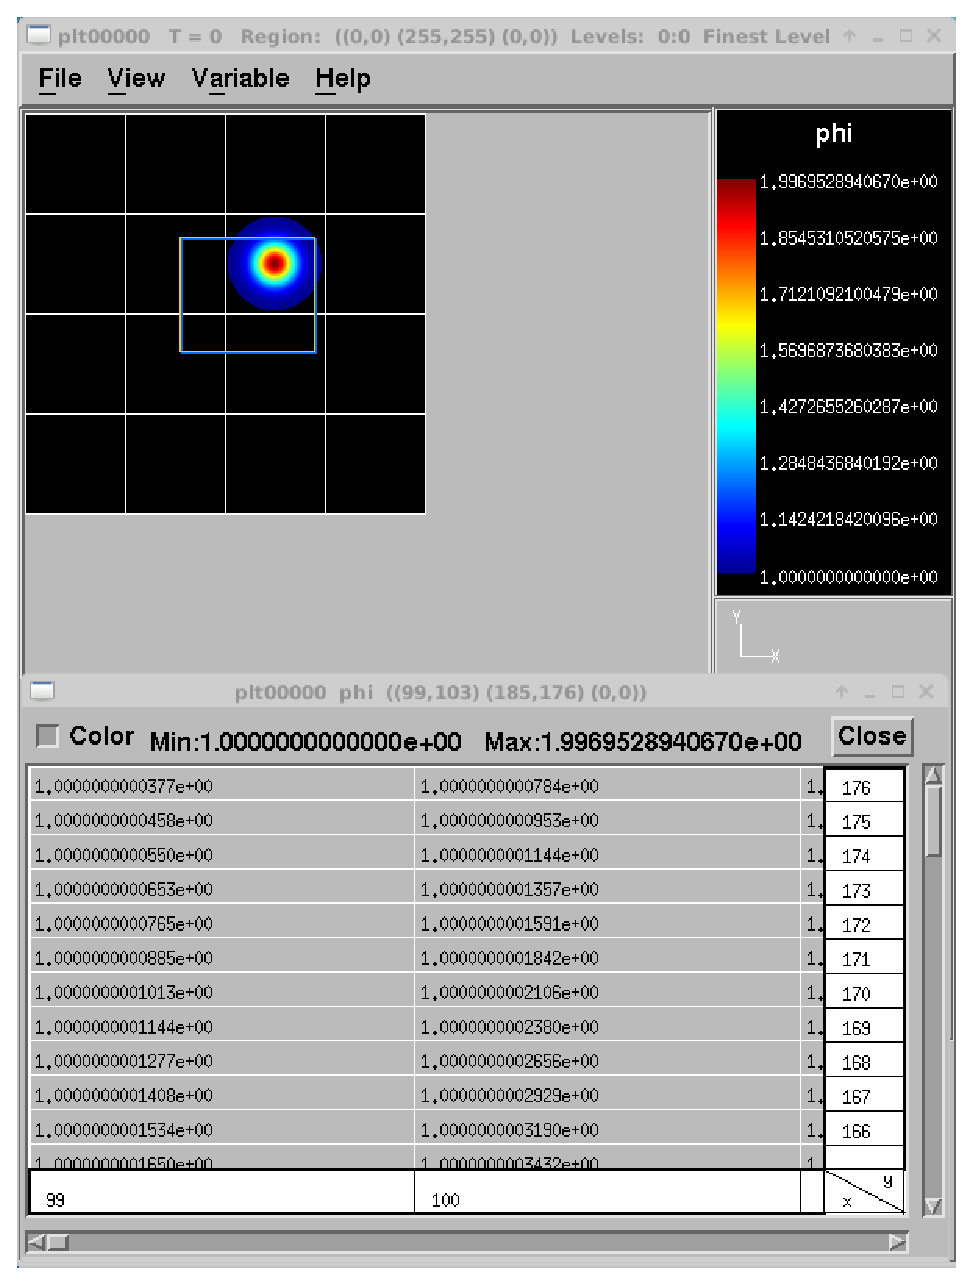
\includegraphics[width=2.5in]{./Visualization/Amrvis_2d}
~~~
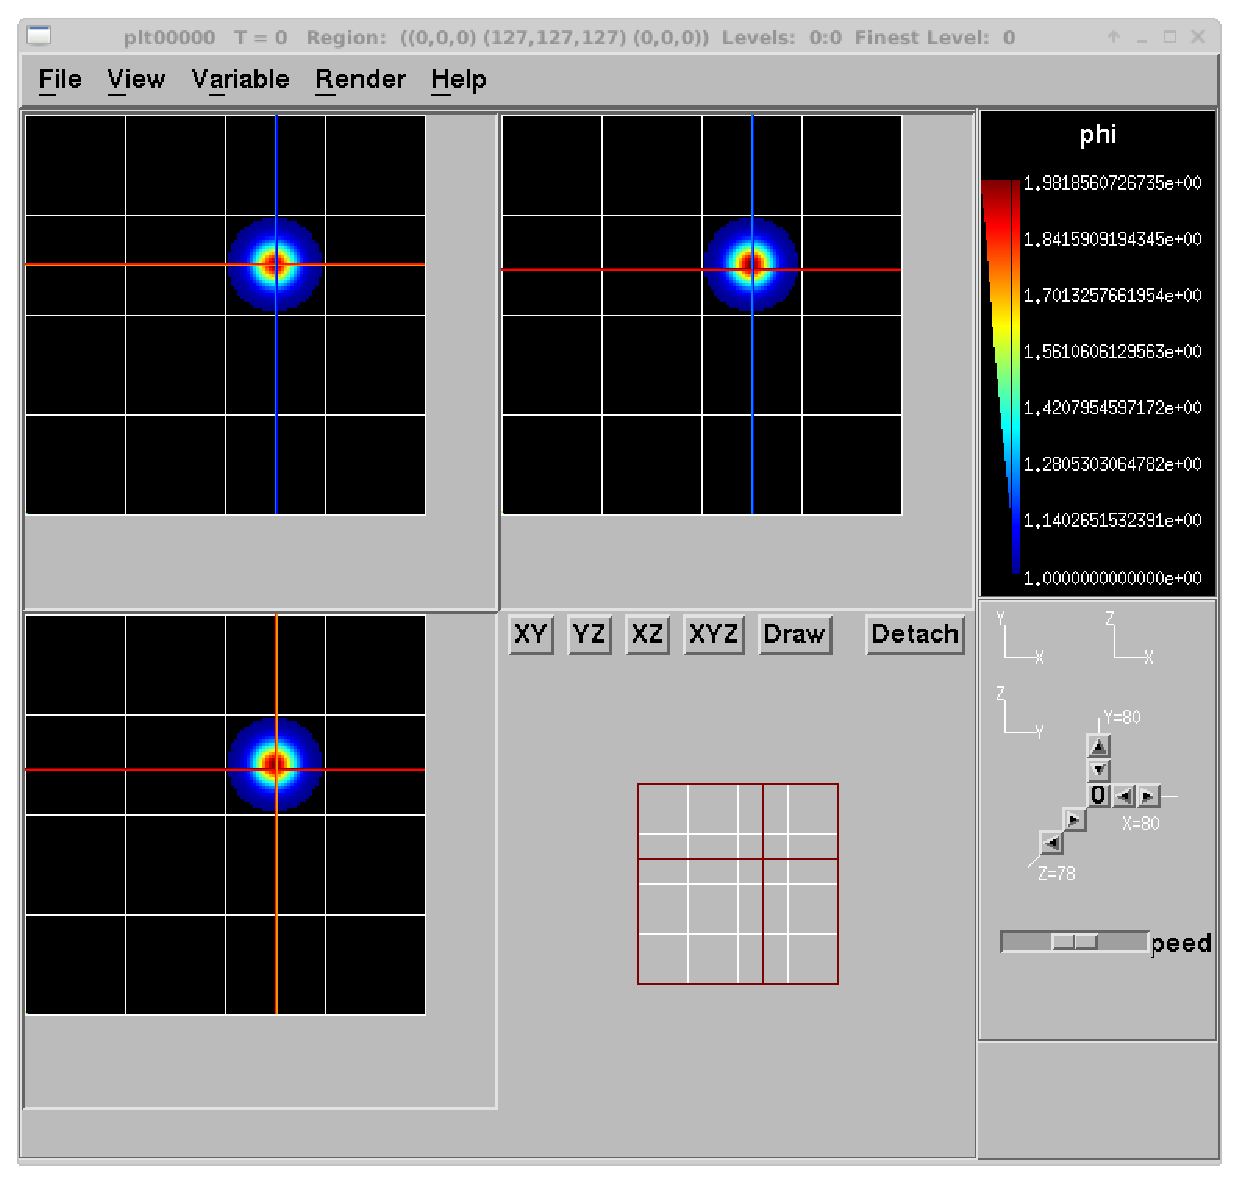
\includegraphics[width=2.5in]{./Visualization/Amrvis_3d}
\caption{2D and 3D images generated with Amrvis}
\label{Fig:Amrvis}
\end{figure}

  We have created a number of routines to convert \amrex\ plotfile data
  other formats (such as matlab), but in order to properly interpret 
  the hierarchical AMR data, each tends to have its own idiosyncrasies.
  If you would like to display the data in another format, please contact
  Marc Day ({\tt MSDay@lbl.gov}) and we will point you to whatever we have
  that can help.

\end{enumerate}

\section{\visit}
\label{sec:visit}

\amrex\ data can also be visualized by {\tt VisIt}, an open
source visualization and analysis software.  To follow along with this example,
first build and run the first heat equation tutorial code
(see Section \ref{sec:heat equation}).

Next, download and install {\tt VisIt} from \url{https://wci.llnl.gov/simulation/computer-codes/visit}.
To open a single plotfile, run {\tt VisIt}, then select ``File'' $\rightarrow$ ``Open file ...'',
then select the {\tt Header} file associated the the plotfile of interest (e.g., {\tt plt00000/Header}).
Assuming you ran the simulation in 2D, here are instructions for making a simple plot:
\begin{itemize}
\item To view the data, select ``Add'' $\rightarrow$ ``Pseudocolor'' $\rightarrow$ ``phi'', and then select
``Draw''.
\item To view the grid structure (not particularly interesting yet, but when we add AMR it will be), select
`` $\rightarrow$ ``subset'' $\rightarrow$ ``levels''.  Then double-click the text ``Subset - levels'',
enable the ``Wireframe'' option, select ``Apply'', select ``Dismiss'', and then select ``Draw''.
\item To save the image, select ``File'' $\rightarrow$ ``Set save options'', then customize the image format
to your liking, then click ``Save''.
\end{itemize}
Your image should look similar to the left side of Figure \ref{Fig:VisIt}.\\
\begin{figure}[tb]
\centering
\includegraphics[width=3.1in]{./Visualization/VisIt_2D}
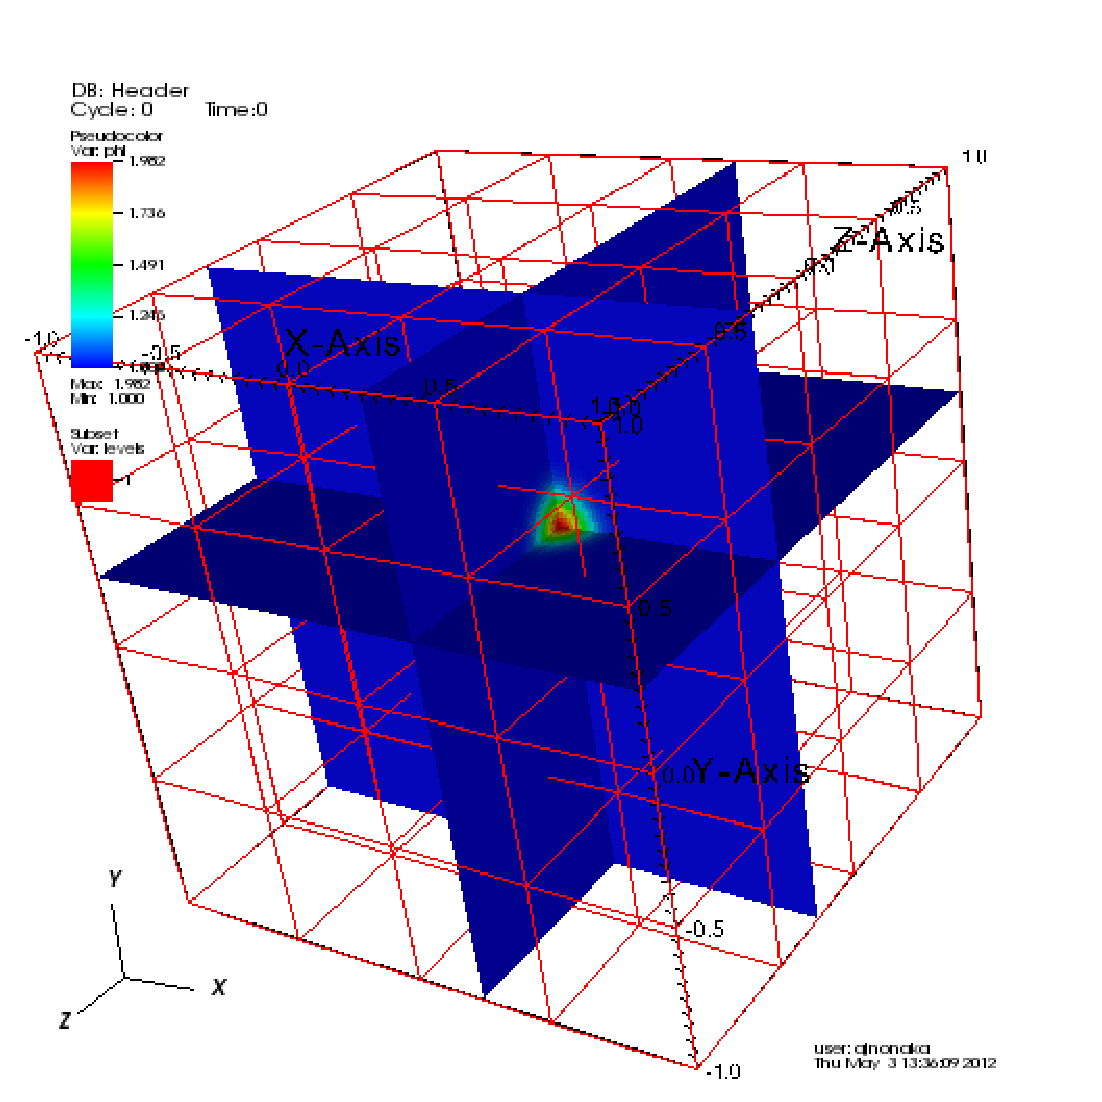
\includegraphics[width=3.1in]{./Visualization/VisIt_3D}
\caption{(Left) 2D image generated with VisIt.  (Right) 3D image generated with VisIt.}
\label{Fig:VisIt}
\end{figure}

In 3D, you must apply the ``Operators'' $\rightarrow$ ``Slicing'' $\rightarrow$ ``ThreeSlice'', with the 
``ThreeSlice operator attribute'' set to x=0.25, y=0.25, and z=0.25.  You can left-click and drag
over the image to rotate the image to generate something similar to right side of Figure \ref{Fig:VisIt}.\\

To make a movie, you must first create a text file named {\tt movie.visit} with a list of the {\tt Header} 
files for the individual frames.  This can most easily be done using the command:
\begin{lstlisting}[backgroundcolor=\color{light-red}]
~/amrex/Tutorials/Basic/HeatEquation_EX1_C> ls -1 plt*/Header | tee movie.visit
plt00000/Header
plt01000/Header
plt02000/Header
plt03000/Header
plt04000/Header
plt05000/Header
plt06000/Header
plt07000/Header
plt08000/Header
plt09000/Header
plt10000/Header
\end{lstlisting}
The next step is to run {\tt VisIt}, select ``File'' $\rightarrow$ ``Open file ...'',
then select {\tt movie.visit}.  Create an image to your liking and press the ``play'' button
on the VCR-like control panel to preview all the frames.  To save the movie, choose
``File'' $\rightarrow$ ``Save movie ...'', and follow the on-screen instructions.

\section{\paraview}
The open source visualization package \paraview\ v5.3.0 can be used to view 
3D plotfiles, and v5.4.0 can be used to view particle data.  Download
the package at \url{https://www.paraview.org/}.  

To open a single plotfile (for example, you could run the {\tt HeatEquation\_EX1\_C} in 3D:
\begin{enumerate}
\item Run \paraview\ v5.3.0, then select ``File'' $\rightarrow$ ``Open''.
\item Navigate to the plotfile directory, and manually type in ``Header''.
      \paraview\ will ask you about the file type -- choose ``Boxlib 3D Files''
\item Under the ``Cell Arrays'' field, select a variable (e.g., ``phi'') 
      and click ``Apply''.
\item Under ``Representation'' select ``Surface''.
\item Under ``Coloring'' select the variable you chose above.
\item To add planes, near the top left you will see a cube icon with a green plane
      slicing through it.  If you hover your mouse over it, it will say ``Slice''.
      Click that button.
\item You can play with the Plane Parameters to define a plane of data to view, as shown
      in Figure \ref{fig:ParaView}.
\end{enumerate}

\begin{figure}[tb]
\centering
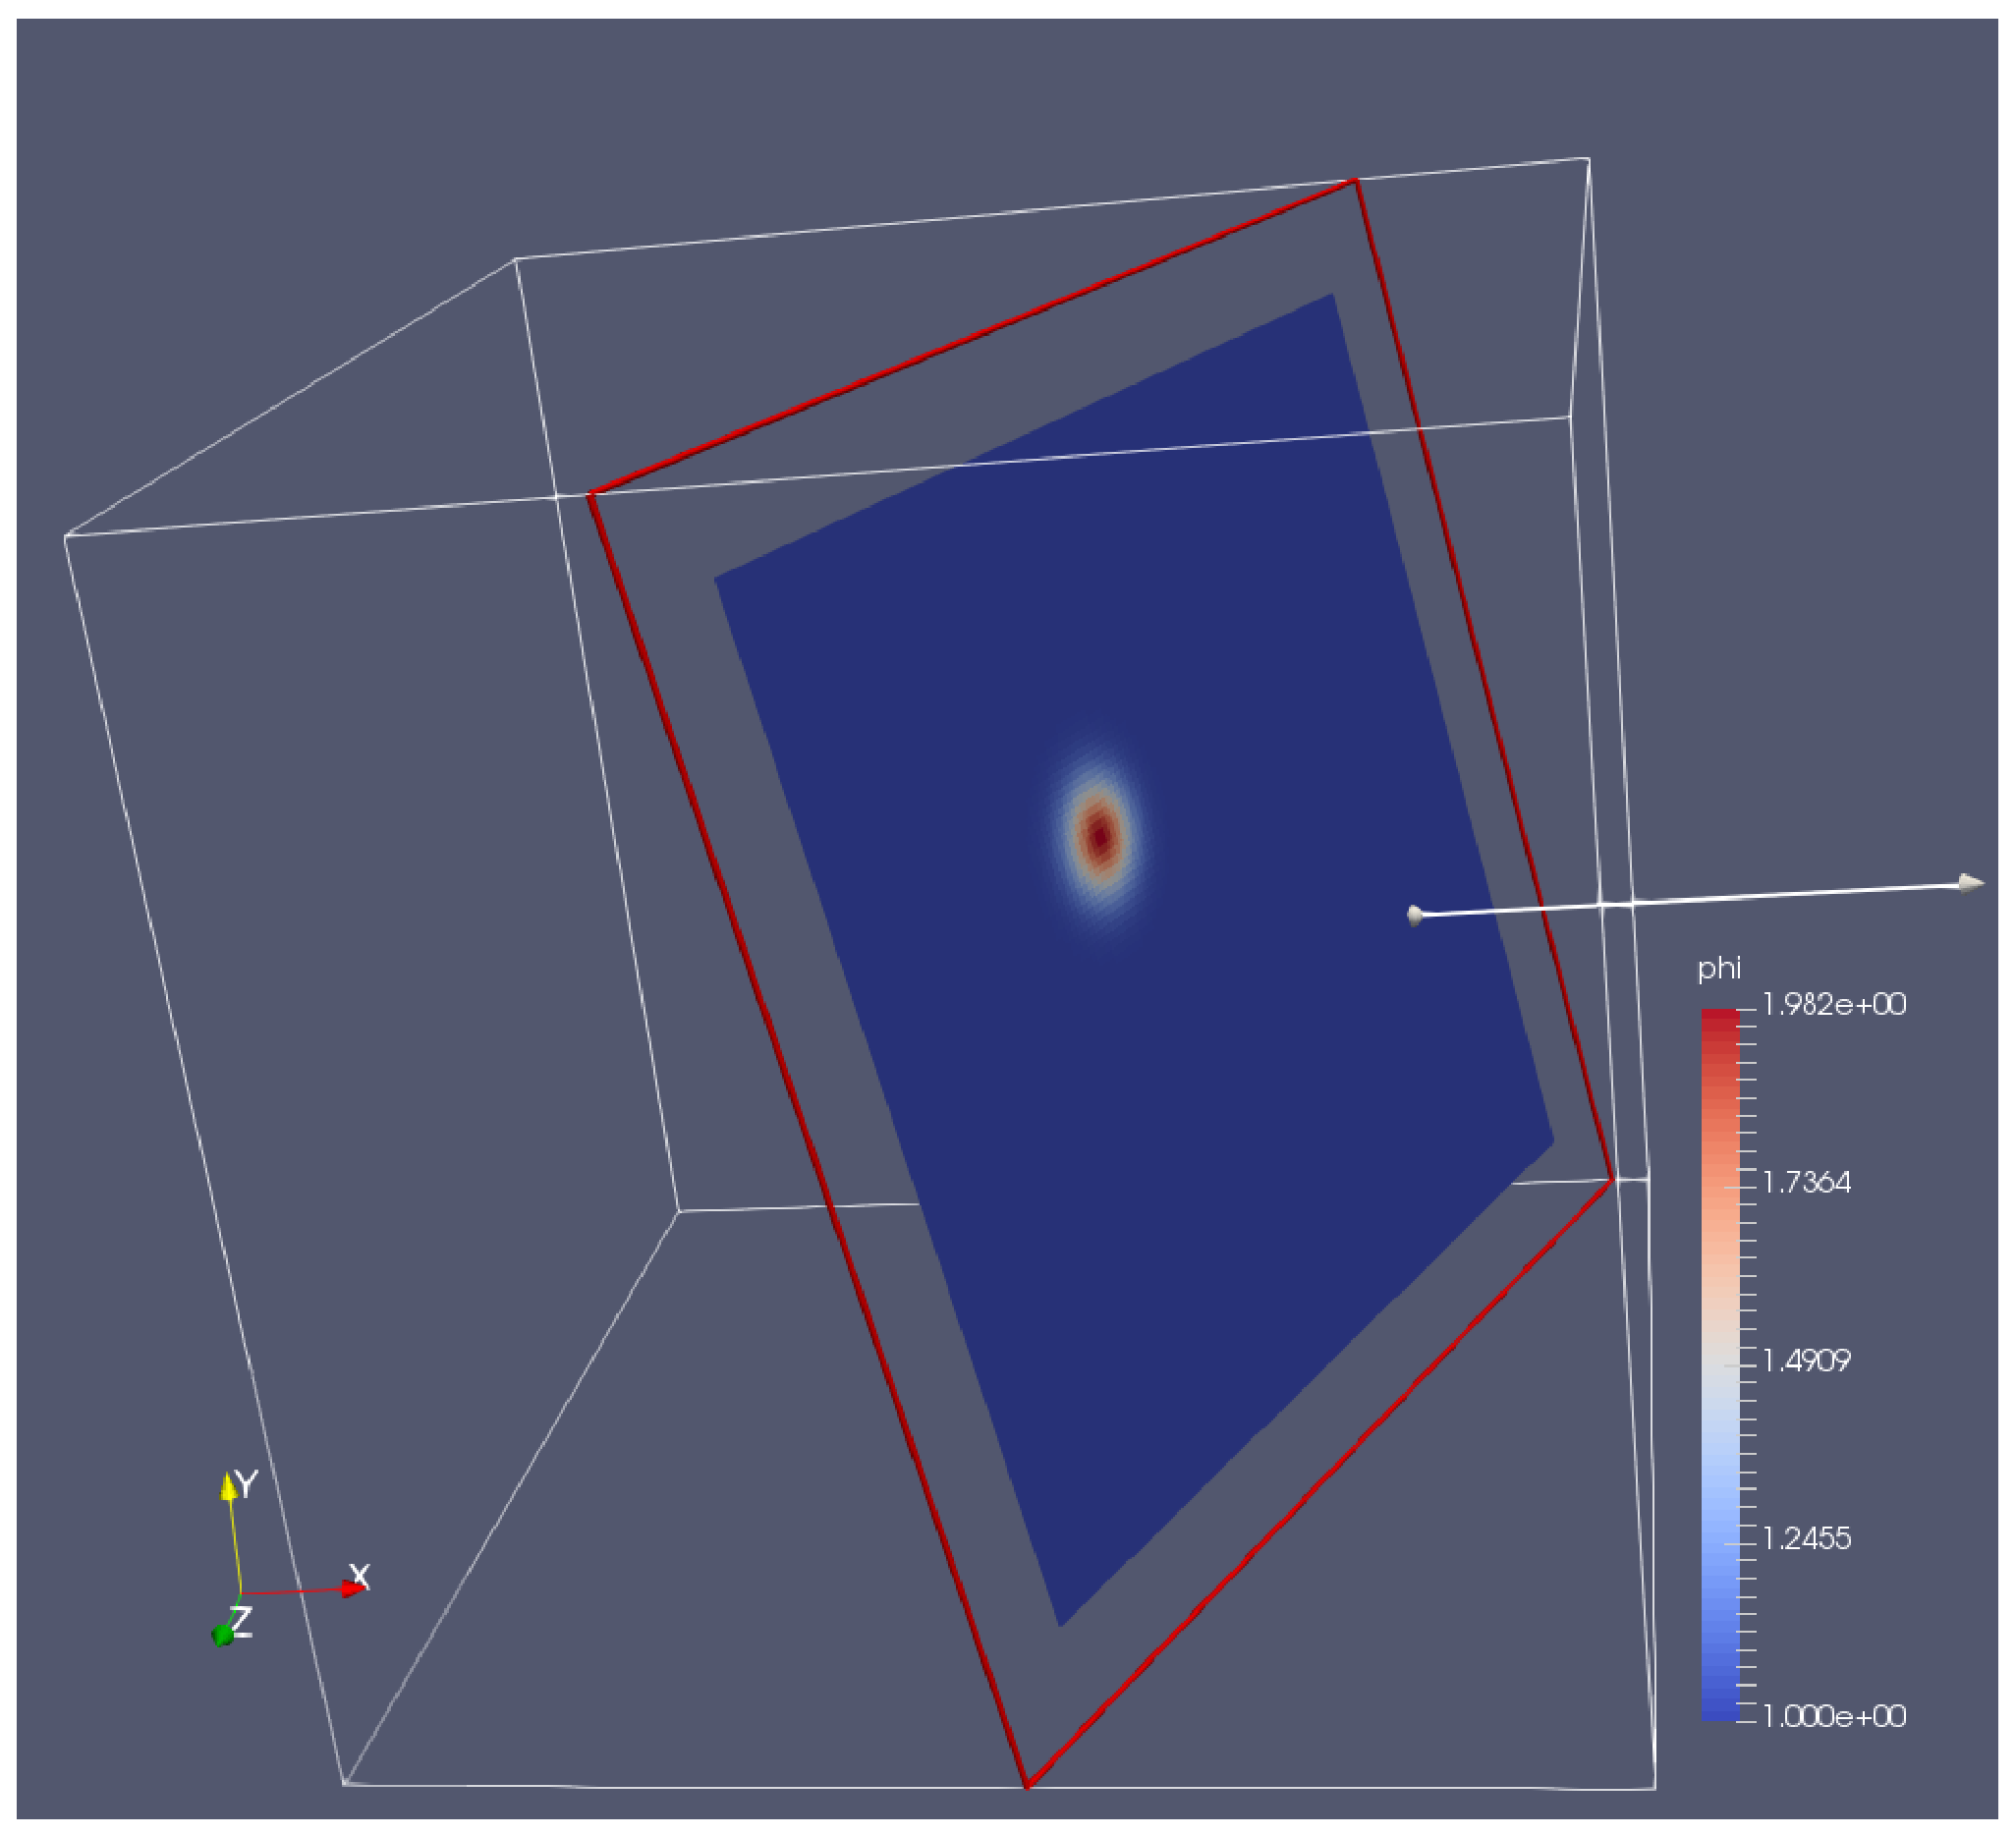
\includegraphics[width=3.1in]{./Visualization/ParaView}
\caption{Plotfile image generated with \paraview}
\label{fig:ParaView}
\end{figure}

To visualize particles (for example, you could run the {\tt ShortRangeParticles} example:
\begin{enumerate}
\item First, we have to convert the \amrex\ particle data to a format \paraview\ can read.
      In the run directory, there will be a sequence of particle files ({\tt particles00000},
      {\tt particles00001}, $\cdots$, {\tt particles01000}).
\item Run the script,
      {\tt amrex/Tools/Py\_util/amrex\_particles\_to\_vtp/amrex\_particles\_to\_vtp.py}
      as follows, e.g.,
      {\tt python amrex\_particles\_to\_vtp.py 0 1000 particles}.  You will generate
      a sequence of {\tt .vtp} files.
\item Run \paraview v5.4.0, and select ``File'' $\rightarrow$ ``Open''.  You will see
      a combined ``particles..vtp'' file grouping the files.  Select that and click OK.
\item Click ``Apply'' and under ``Representation'' select ``Point Gaussian''.
\item Change the Gaussian Radius if you like.  You can scroll through the frames with the
      VCR-like controls at the top, as shown in Figure \ref{fig:ParaView_particles}.
\end{enumerate}


\begin{figure}[tb]
\centering
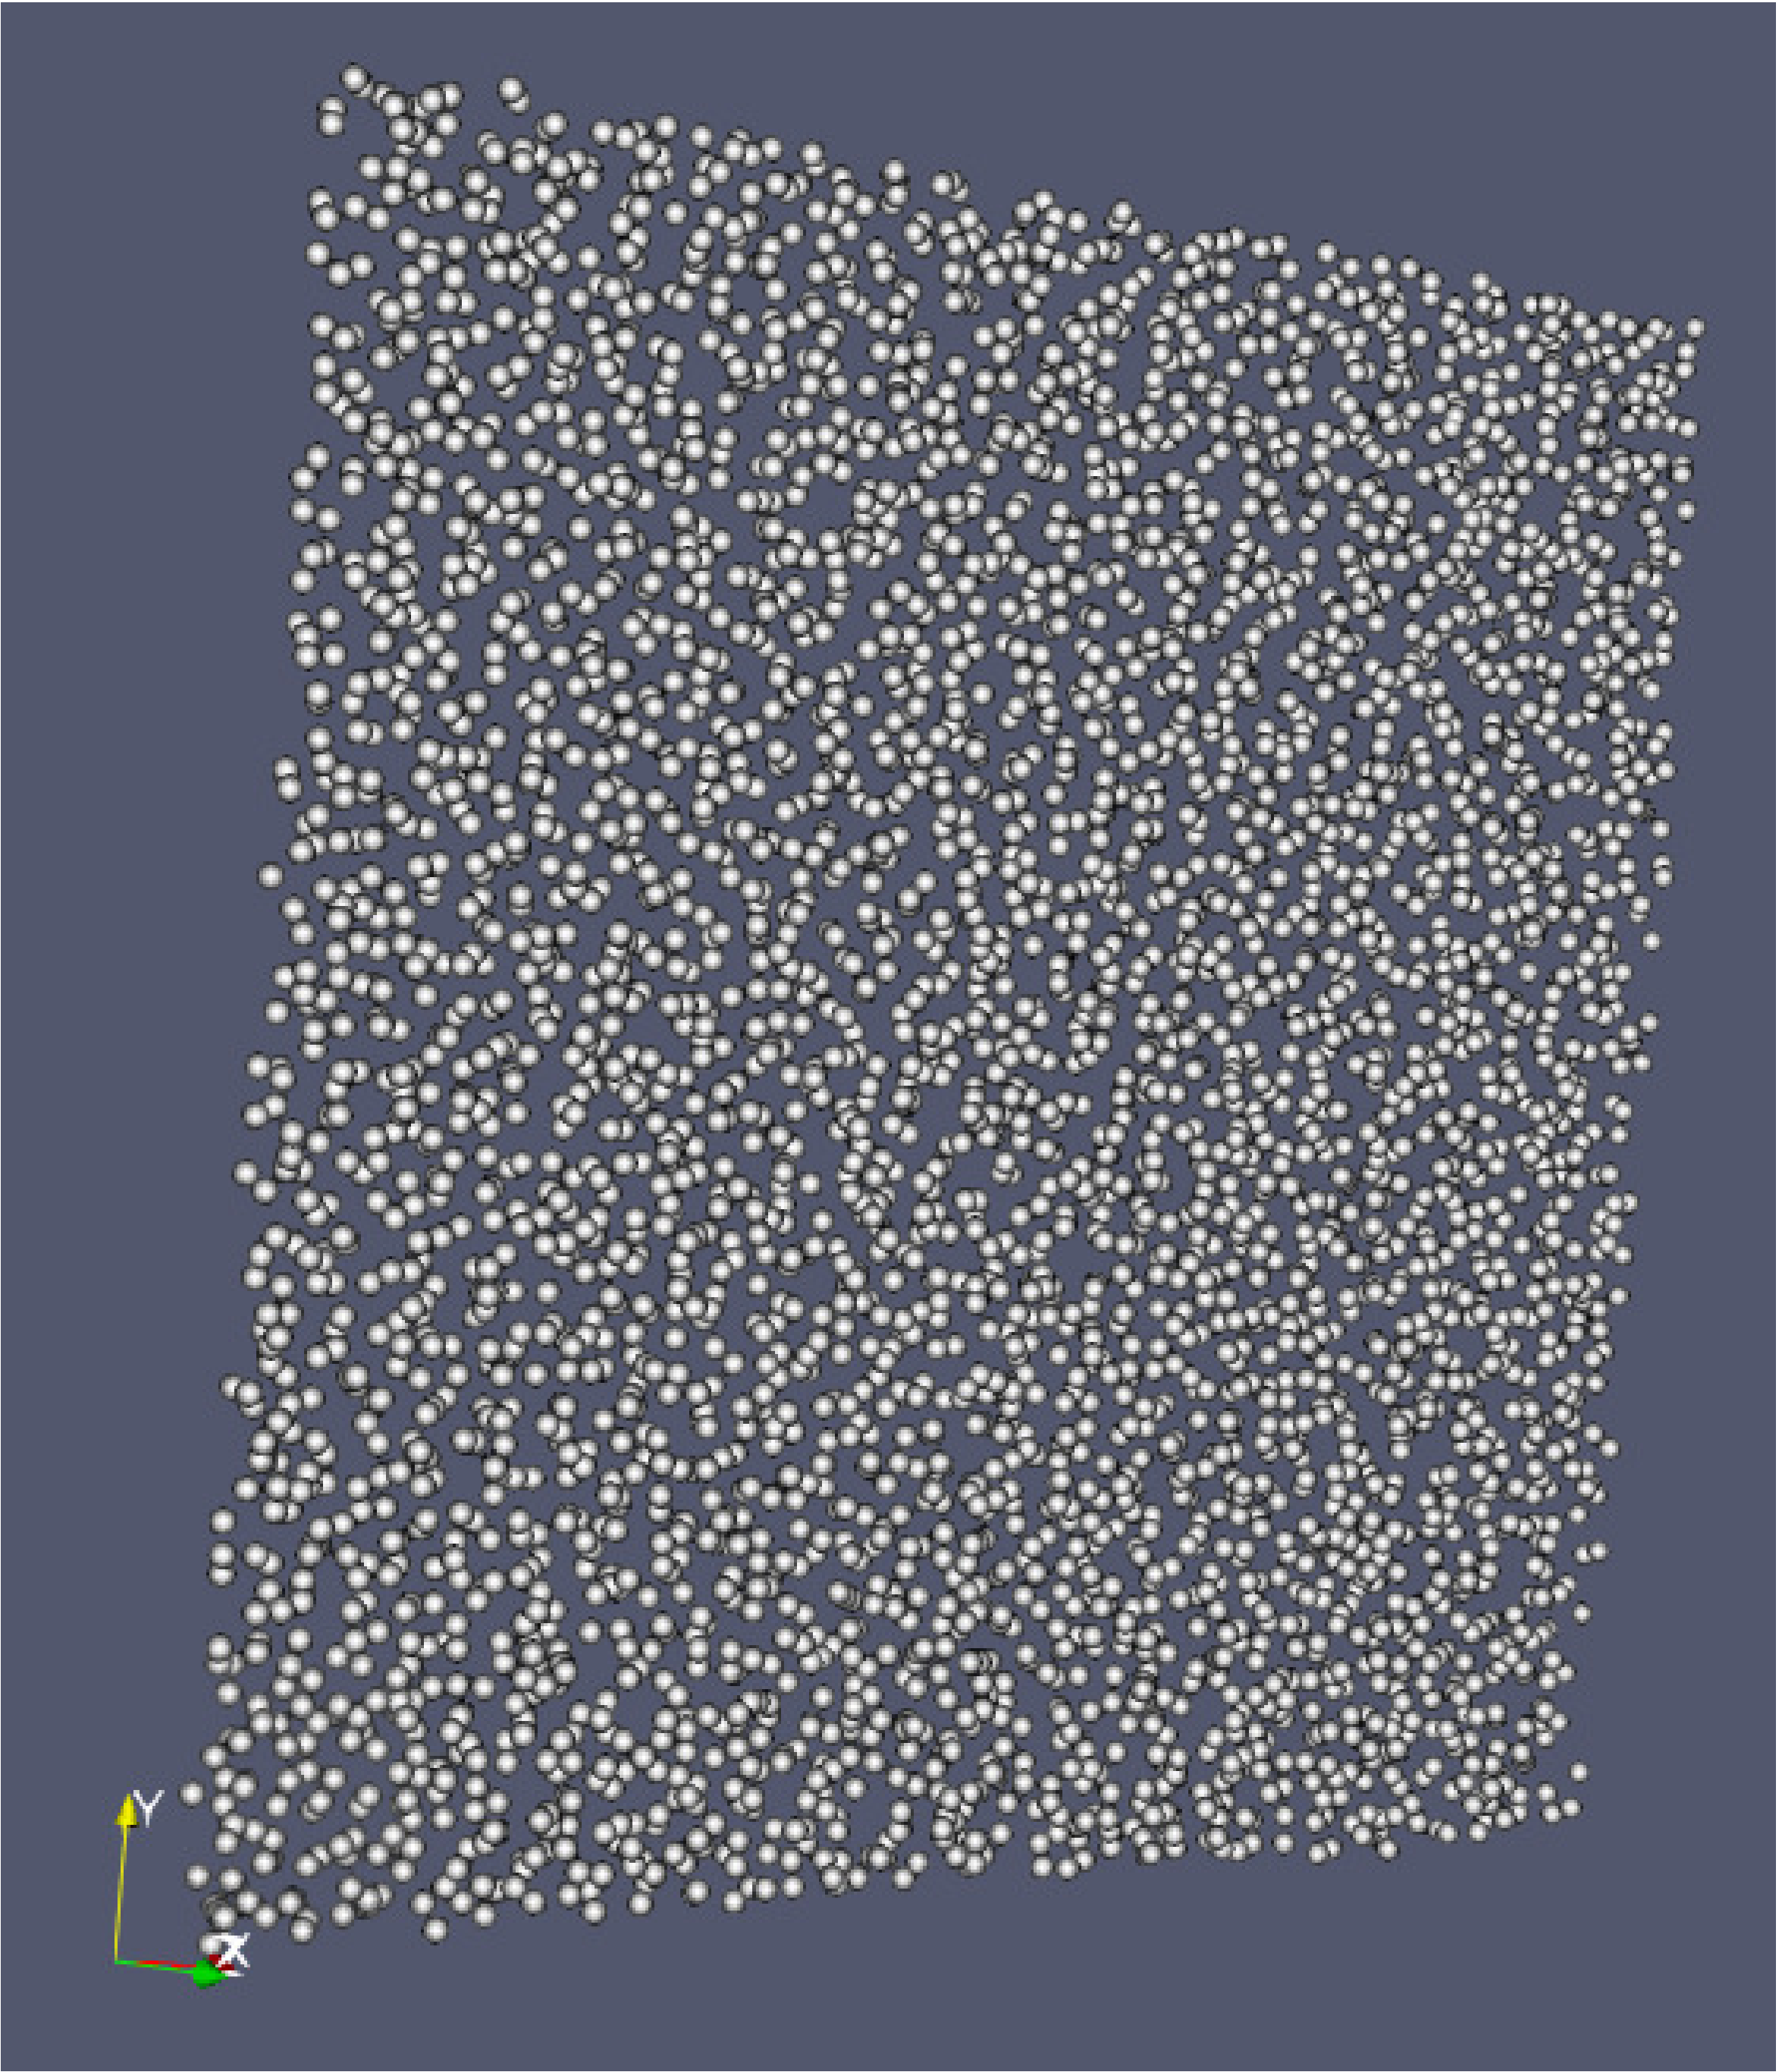
\includegraphics[width=3.1in]{./Visualization/ParaView_particles}
\caption{Particle image generated with \paraview}
\label{fig:ParaView_particles}
\end{figure}

\section{\yt}

\yt, an open source Python package available at \url{http://yt-project.org/},
can be used for analyzing and visualizing mesh and particle data generated by
\amrex\ codes.  Some of the \amrex\ developers are also \yt\ project members.
Below we describe how to use \yt\ on both a local workstation, as well as at
the NERSC HPC facility for high-throughput visualization of large data sets.

\subsection{Using \yt\ on a local workstation}

Running \yt\ on a local system generally provides good interactivity, but
limited performance. Consequently, this configuration is best when doing
exploratory visualization (e.g., experimenting with camera angles, lighting,
and color schemes) of small data sets.

To use \yt\ on an \amrex\ plot file, first start a Jupyter notebook or an IPython kernel, and import the \texttt{yt} module:

\begin{lstlisting}[language=python,breaklines=true]
In [1]: import yt

In [2]: print(yt.__version__)
3.4-dev
\end{lstlisting}

Next, load a plot file; in this example we use a plot file from the Nyx cosmology application:

\begin{lstlisting}[language=python,breaklines=true]
In [3]: ds = yt.load("plt00401")
yt : [INFO     ] 2017-05-23 10:03:56,182 Parameters: current_time              = 0.00605694344696544
yt : [INFO     ] 2017-05-23 10:03:56,182 Parameters: domain_dimensions         = [128 128 128]
yt : [INFO     ] 2017-05-23 10:03:56,182 Parameters: domain_left_edge          = [ 0.  0.  0.]
yt : [INFO     ] 2017-05-23 10:03:56,183 Parameters: domain_right_edge         = [ 14.24501  14.24501  14.24501]

In [4]: ds.field_list
Out[4]:
[('DM', 'particle_mass'),
 ('DM', 'particle_position_x'),
 ('DM', 'particle_position_y'),
 ('DM', 'particle_position_z'),
 ('DM', 'particle_velocity_x'),
 ('DM', 'particle_velocity_y'),
 ('DM', 'particle_velocity_z'),
 ('all', 'particle_mass'),
 ('all', 'particle_position_x'),
 ('all', 'particle_position_y'),
 ('all', 'particle_position_z'),
 ('all', 'particle_velocity_x'),
 ('all', 'particle_velocity_y'),
 ('all', 'particle_velocity_z'),
 ('boxlib', 'density'),
 ('boxlib', 'particle_mass_density')]
\end{lstlisting}

From here one can make slice plots, 3-D volume renderings, etc. An example of
the slice plot feature is shown below:

\begin{lstlisting}[language=python,breaklines=true]
In [9]: slc = yt.SlicePlot(ds, "z", "density")
yt : [INFO     ] 2017-05-23 10:08:25,358 xlim = 0.000000 14.245010
yt : [INFO     ] 2017-05-23 10:08:25,358 ylim = 0.000000 14.245010
yt : [INFO     ] 2017-05-23 10:08:25,359 xlim = 0.000000 14.245010
yt : [INFO     ] 2017-05-23 10:08:25,359 ylim = 0.000000 14.245010

In [10]: slc.show()

In [11]: slc.save()
yt : [INFO     ] 2017-05-23 10:08:34,021 Saving plot plt00401_Slice_z_density.png
Out[11]: ['plt00401_Slice_z_density.png']
\end{lstlisting}

The resulting image is Figure~\ref{fig:yt_Nyx_slice_plot}. One can also make
volume renderings with \yt; an example is show below:

\begin{figure}
  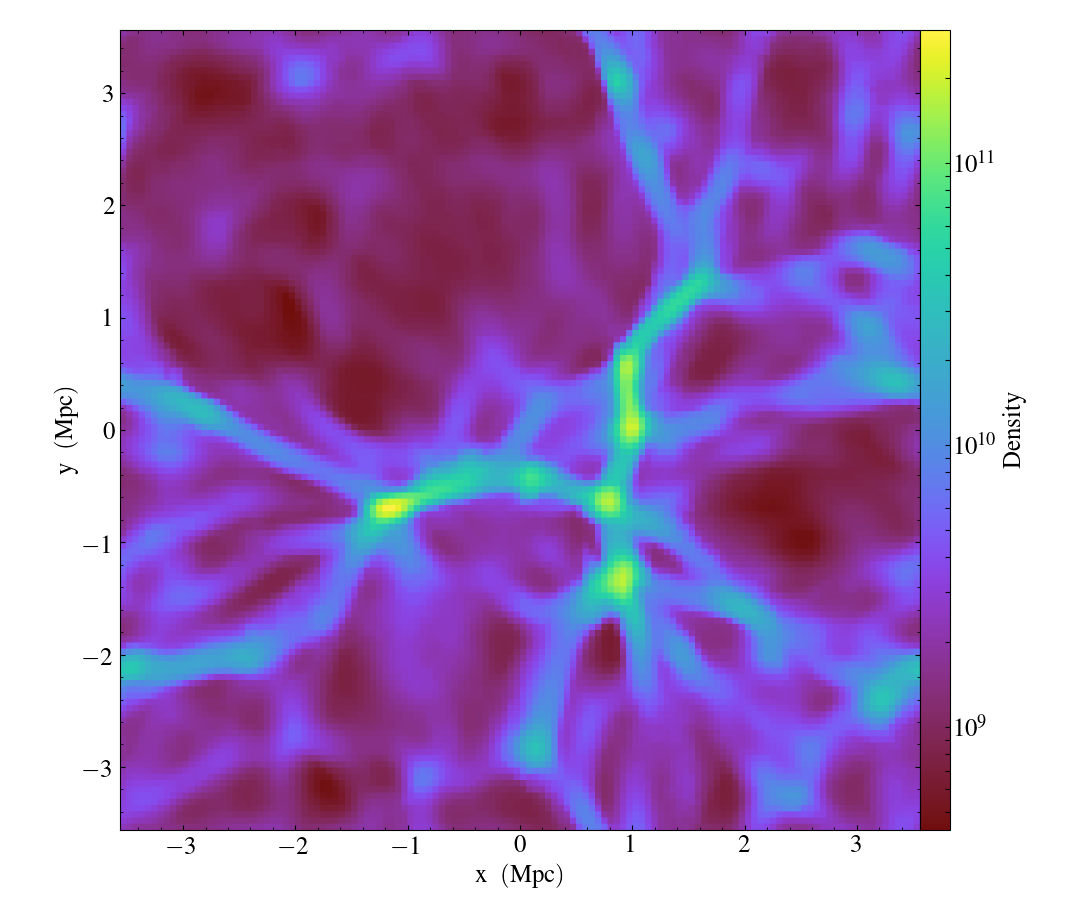
\includegraphics[scale=0.5]{./Visualization/yt_Nyx_density_slice.png}
  \caption{Slice plot of $128^3$ Nyx simulation using \yt.}
  \label{fig:yt_Nyx_slice_plot}
\end{figure}

\begin{lstlisting}[language=python,breaklines=true]
In [12]: sc = yt.create_scene(ds, field="density", lens_type="perspective")

In [13]: source = sc[0]

In [14]: source.tfh.set_bounds((1e8, 1e15))

In [15]: source.tfh.set_log(True)

In [16]: source.tfh.grey_opacity = True

In [17]: sc.show()
<Scene Object>:
Sources:
    source_00: <Volume Source>:YTRegion (plt00401): , center=[  1.09888770e+25   1.09888770e+25   1.09888770e+25] cm, left_edge=[ 0.  0.  0.] cm, right_edge=[  2.19777540e+25   2.19777540e+25   2.19777540e+25] cm transfer_function:None
Camera:
    <Camera Object>:
	position:[ 14.24501  14.24501  14.24501] code_length
	focus:[ 7.122505  7.122505  7.122505] code_length
	north_vector:[ 0.81649658 -0.40824829 -0.40824829]
	width:[ 21.367515  21.367515  21.367515] code_length
	light:None
	resolution:(512, 512)
Lens: <Lens Object>:
	lens_type:perspective
	viewpoint:[ 0.95423473  0.95423473  0.95423473] code_length

In [19]: sc.save()
yt : [INFO     ] 2017-05-23 10:15:07,825 Rendering scene (Can take a while).
yt : [INFO     ] 2017-05-23 10:15:07,825 Creating volume
yt : [INFO     ] 2017-05-23 10:15:07,996 Creating transfer function
yt : [INFO     ] 2017-05-23 10:15:07,997 Calculating data bounds. This may take a while.  
Set the TransferFunctionHelper.bounds to avoid this.
yt : [INFO     ] 2017-05-23 10:15:16,471 Saving render plt00401_Render_density.png
\end{lstlisting}

The output of this is Figure~\ref{fig:yt_Nyx_vol_rend}.

\begin{figure}
  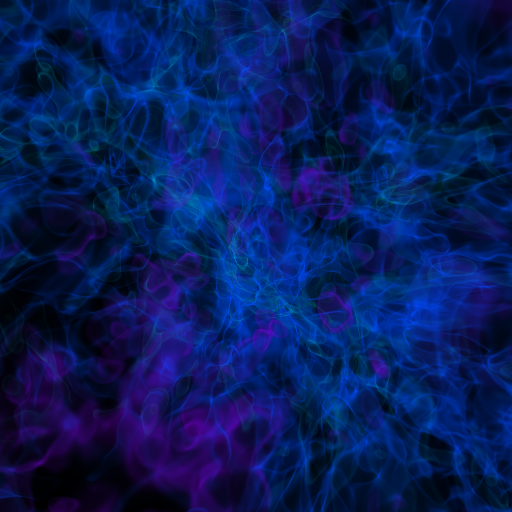
\includegraphics[scale=1.0]{./Visualization/yt_Nyx_density_vol_rend.png}
  \caption{Volume rendering of $128^3$ Nyx simulation using \yt. This
           corresponds to the same plot file used to generate the slice plot in
           Figure~\ref{fig:yt_Nyx_slice_plot}.}
  \label{fig:yt_Nyx_vol_rend}
\end{figure}

\subsection{Using \yt\ at NERSC (\emph{under development})}

Because \yt\ is Python-based, it is portable and can be used in many software
environments. Here we focus on \yt's capabilities at NERSC, which provides
resources for performing both interactive and batch queue-based visualization
and analysis of \amrex\ data. Coupled with \yt's MPI and OpenMP parallelization
capabilities, this can enable high-throughput visualization and analysis
workflows.

\subsubsection{Interactive \yt\ with Jupyter notebooks}

Unlike \visit\ (\S\ref{sec:visit}), \yt\ has no client-server interface. Such
an interface is often crucial when one has large data sets generated on a
remote system, but wishes to visualize the data on a local workstation. Both
copying the data between the two systems, as well as visualizing the data
itself on a workstation, can be prohibitively slow.

Fortunately, NERSC has implemented several resources which allow one to
interact with \yt\ remotely, emulating a client-server model. In particular,
NERSC now hosts Jupyter notebooks which run IPython kernels on the Cori system;
this provides users access to the \texttt{\$HOME}, \texttt{/project}, and
\texttt{\$SCRATCH} file systems from a web browser-based Jupyter notebook.
\emph{\textbf{Please note that Jupyter hosting at NERSC is still under
development, and the environment may change without notice.}}

NERSC also provides Anaconda Python, which allows users to create their own
customizable Python environments. It is recommended to install \yt\ in such an
environment. One can do so with the following example:

\begin{lstlisting}
user@cori10:~> module load python/3.5-anaconda
user@cori10:~> conda create -p $HOME/yt-conda numpy
user@cori10:~> source activate $HOME/yt-conda
(/global/homes/u/user/yt-conda/) user@cori10:~> pip install yt
\end{lstlisting}

More information about Anaconda Python at NERSC is here:
\url{http://www.nersc.gov/users/data-analytics/data-analytics/python/anaconda-python/}.

One can then configure this Anaconda environment to run in a Jupyter notebook
hosted on the Cori system. Currently this is available in two places: on
\url{https://ipython.nersc.gov}, and on \url{https://jupyter-dev.nersc.gov}.
The latter likely reflects what the stable, production environment for Jupyter
notebooks will look like at NERSC, but it is still under development and
subject to change. To load this custom Python kernel in a Jupyter notebook,
follow the instructions at this URL under the ``Custom Kernels'' heading:
\url{http://www.nersc.gov/users/data-analytics/data-analytics/web-applications-for-data-analytics}.
After writing the appropriate \texttt{kernel.json} file, the custom kernel will
appear as an available Jupyter notebook. Then one can interactively visualize
\amrex\ plot files in the web browser.\footnote{It is convenient to use the
magic command \texttt{\%matplotlib inline} in order to render matplotlib
figures in the same browser window as the notebook, as opposed to displaying it
as a new window.}

\subsubsection{Parallel \yt}

Besides the benefit of no longer needing to move data back and forth between
NERSC and one's local workstation to do visualization and analysis, an
additional feature of \yt\ which takes advantage of the computational resources
at NERSC is its parallelization capabilities. \yt\ supports both MPI- and
OpenMP-based parallelization of various tasks, which are discussed here:
\url{http://yt-project.org/doc/analyzing/parallel_computation.html}.

Configuring \yt\ for MPI parallelization at NERSC is a more complex task than
discussed on the official \yt\ documentation; the command \texttt{pip install
mpi4py} is not sufficient. Rather, one must compile \texttt{mpi4py} from source
using the Cray compiler wrappers \texttt{cc}, \texttt{CC}, and \texttt{ftn} on
Cori. Instructions for compiling \texttt{mpi4py} at NERSC are provided here:
\url{http://www.nersc.gov/users/data-analytics/data-analytics/python/anaconda-python/#toc-anchor-3}.
After \texttt{mpi4py} has been compiled, one can use the regular Python
interpreter in the Anaconda environment as normal; when executing \yt\
operations which support MPI parallelization, the multiple MPI processes will
spawn automatically.

Although several components of \yt\ support MPI parallelization, a few are particularly useful:
\begin{itemize}
  \item \textbf{Time series analysis.} Often one runs a simulation for many
time steps and periodically writes plot files to disk for visualization and
post-processing. \yt\ supports parallelization over time series data via the
\texttt{DatasetSeries} object. \yt\ can iterate over a \texttt{DatasetSeries}
in parallel, with different MPI processes operating on different elements of
the series. This page provides more documentation:
\url{http://yt-project.org/doc/analyzing/time_series_analysis.html#time-series-analysis}.

  \item \textbf{Volume rendering}. \yt\ implements spatial decomposition among
MPI processes for volume rendering procedures, which can be computationally
expensive. Note that \yt\ also implements OpenMP parallelization in volume
rendering, and so one can execute volume rendering with a hybrid MPI+OpenMP
approach. See this URL for more detail:
\url{http://yt-project.org/doc/visualizing/volume_rendering.html?highlight=openmp#openmp-parallelization}.

  \item \textbf{Generic parallelization over multiple objects.} Sometimes one
wishes to loop over a series which is not a \texttt{DatasetSeries}, e.g.,
performing translational or rotational operations on a camera to make a volume
rendering in which the field of view moves through the simulation. In this
case, one is applying a set of operations on a single object (a single plot
file), rather than over a time series of data. For this workflow, \yt\ provides
the \texttt{parallel\_objects()} function. See this URL for more details:
\url{http://yt-project.org/doc/analyzing/parallel_computation.html#parallelizing-over-multiple-objects}.

An example of MPI parallelization in \yt\ is shown below, where one animates a
time series of plot files from an IAMR simulation while revolving the camera
such that it completes two full revolutions over the span of the animation:

\begin{lstlisting}[language=python,breaklines=true]
import yt
import glob
import numpy as np

yt.enable_parallelism()

base_dir1 = '/global/cscratch1/sd/user/Nyx_run_p1'
base_dir2 = '/global/cscratch1/sd/user/Nyx_run_p2'
base_dir3 = '/global/cscratch1/sd/user/Nyx_run_p3'

glob1 = glob.glob(base_dir1 + '/plt*')
glob2 = glob.glob(base_dir2 + '/plt*')
glob3 = glob.glob(base_dir3 + '/plt*')

files = sorted(glob1 + glob2 + glob3)

ts = yt.DatasetSeries(files, parallel=True)

frame = 0
num_frames = len(ts)
num_revol = 2

slices = np.arange(len(ts))

for i in yt.parallel_objects(slices):
    sc = yt.create_scene(ts[i], lens_type='perspective', field='z_velocity')

    source = sc[0]
    source.tfh.set_bounds((1e-2, 9e+0))
    source.tfh.set_log(False)
    source.tfh.grey_opacity = False

    cam = sc.camera

    cam.rotate(num_revol*(2.0*np.pi)*(i/num_frames),
               rot_center=np.array([0.0, 0.0, 0.0]))

    sc.save(sigma_clip=5.0)
\end{lstlisting}

When executed on 4 CPUs on a Haswell node of Cori, the output looks like the following:

\begin{lstlisting}[breaklines=true]
user@nid00009:~/yt_vis/> srun -n 4 -c 2 --cpu_bind=cores python make_yt_movie.py
yt : [INFO     ] 2017-05-23 16:51:33,565 Global parallel computation enabled: 0 / 4
yt : [INFO     ] 2017-05-23 16:51:33,565 Global parallel computation enabled: 2 / 4
yt : [INFO     ] 2017-05-23 16:51:33,566 Global parallel computation enabled: 1 / 4
yt : [INFO     ] 2017-05-23 16:51:33,566 Global parallel computation enabled: 3 / 4
P003 yt : [INFO     ] 2017-05-23 16:51:33,957 Parameters: current_time              = 0.103169376949795
P003 yt : [INFO     ] 2017-05-23 16:51:33,957 Parameters: domain_dimensions         = [128 128 128]
P003 yt : [INFO     ] 2017-05-23 16:51:33,957 Parameters: domain_left_edge          = [ 0.  0.  0.]
P003 yt : [INFO     ] 2017-05-23 16:51:33,958 Parameters: domain_right_edge         = [ 6.28318531  6.28318531  6.28318531]
P000 yt : [INFO     ] 2017-05-23 16:51:33,969 Parameters: current_time              = 0.0
P000 yt : [INFO     ] 2017-05-23 16:51:33,969 Parameters: domain_dimensions         = [128 128 128]
P002 yt : [INFO     ] 2017-05-23 16:51:33,969 Parameters: current_time              = 0.0687808060674485
P000 yt : [INFO     ] 2017-05-23 16:51:33,969 Parameters: domain_left_edge          = [ 0.  0.  0.]
P002 yt : [INFO     ] 2017-05-23 16:51:33,969 Parameters: domain_dimensions         = [128 128 128]
P000 yt : [INFO     ] 2017-05-23 16:51:33,970 Parameters: domain_right_edge         = [ 6.28318531  6.28318531  6.28318531]
P002 yt : [INFO     ] 2017-05-23 16:51:33,970 Parameters: domain_left_edge          = [ 0.  0.  0.]
P002 yt : [INFO     ] 2017-05-23 16:51:33,970 Parameters: domain_right_edge         = [ 6.28318531  6.28318531  6.28318531]
P001 yt : [INFO     ] 2017-05-23 16:51:33,973 Parameters: current_time              = 0.0343922351851018
P001 yt : [INFO     ] 2017-05-23 16:51:33,973 Parameters: domain_dimensions         = [128 128 128]
P001 yt : [INFO     ] 2017-05-23 16:51:33,974 Parameters: domain_left_edge          = [ 0.  0.  0.]
P001 yt : [INFO     ] 2017-05-23 16:51:33,974 Parameters: domain_right_edge         = [ 6.28318531  6.28318531  6.28318531]
P000 yt : [INFO     ] 2017-05-23 16:51:34,589 Rendering scene (Can take a while).
P000 yt : [INFO     ] 2017-05-23 16:51:34,590 Creating volume
P003 yt : [INFO     ] 2017-05-23 16:51:34,592 Rendering scene (Can take a while).
P002 yt : [INFO     ] 2017-05-23 16:51:34,592 Rendering scene (Can take a while).
P003 yt : [INFO     ] 2017-05-23 16:51:34,593 Creating volume
P002 yt : [INFO     ] 2017-05-23 16:51:34,593 Creating volume
P001 yt : [INFO     ] 2017-05-23 16:51:34,606 Rendering scene (Can take a while).
P001 yt : [INFO     ] 2017-05-23 16:51:34,607 Creating volume
\end{lstlisting}

Because the \texttt{parallel\_objects()} function transforms the loop into a
data-parallel problem, this procedure strong scales nearly perfectly to an
arbitrarily large number of MPI processes, allowing for rapid rendering of
large time series of data.

\end{itemize}


%------------------------------------------------------------------------------
\backmatter

% \renewcommand\bibname{References}
% \addcontentsline{toc}{chapter}{References}
% \bibliographystyle{plain}
% \bibliography{refs,Verification/verification,Gravity/gr}

\cleardoublepage
\phantomsection
\addcontentsline{toc}{chapter}{Index}
\printindex

\end{document}
